\chapter{التطبيق خطوة بخطوة}
\label{ch:walkthrough}

\section{ابدأ من هنا: ما الذي سنبنيه؟}
\label{sec:start}

لنفترض أن لدينا مؤسسة اسمها «وزارة الاقتصاد والصناعة». تتبع لها «الإدارة العامة للتجارة الداخلية وحماية المستهلك»، وتحتها «مديرية حماية المستهلك وسلامة الغذاء»، ثم «دائرة حماية المستهلك». يعمل أحمد ونور وريم في هذه الدائرة.

المشكلة بسيطة: يضيف نور ملف منشأة جديدة، فلا يعرف أحمد بها إلا مصادفة. سنبني «إجراءً داخلياً»، أي سلسلة خطوات يشغّلها النظام وحده، فيبلّغ أحمد ويطلب موافقته، ثم يكلّف نور بالكشف الأول إذا وافق. لن نبنيه دفعة واحدة؛ سنبنيه على أربع مراحل صغيرة، وفي نهاية كل مرحلة تجرّبه فعلاً وترى نتيجته.

\begin{figure}[H]
\centering
\begin{tikzpicture}[node distance=0.5cm]
\node[stepBox] (a) {\RL{المرحلة 1: إشعار واحد إلى أحمد}};
\node[stepBox,below=of a] (b) {\RL{المرحلة 2: أحمد يوافق أو يطلب تغييرات}};
\node[stepBox,below=of b] (c) {\RL{المرحلة 3: طريقان بحسب رده}};
\node[stepBox,below=of c] (d) {\RL{المرحلة 4: مهمة لنور وتحديث الملف}};
\draw[flowsTo] (a) -- (b);
\draw[flowsTo] (b) -- (c);
\draw[flowsTo] (c) -- (d);
\end{tikzpicture}
\rclegend
\caption{أربع مراحل، وكل مرحلة تعمل وحدها}
\label{fig:stages}
\shotnote{كل مرحلة تضيف شيئاً واحداً إلى الإجراء نفسه، ثم تنشره وتجرّبه. لذلك إذا توقفت عند أي مرحلة، يبقى لديك إجراء يعمل، وتعرف بالضبط أين وقع الخطأ إن ظهر.}
\end{figure}

\begin{table}[H]
\centering
\caption{الفريق ودور كل شخص}
\label{tab:team}
\begin{tabularx}{\linewidth}{R{3.5cm} Y Y}
\rcHeaderRow
\thh{الشخص} & \thh{المنصب} & \thh{دوره في هذا الفصل}\\
أحمد سالم — تجريبي & رئيس فريق الكشف الميداني — 01 & يصله الإشعار، ويرد على طلب الموافقة.\\
نور حسن — تجريبي & باحث ميداني — 01 & يضيف المنشأة، وتصله مهمة الكشف الأول أو طلب الاستكمال.\\
ريم خالد — تجريبي & مدقق كشوف المنشآت — 01 & نضيفها في تمرين الإتقان آخر الفصل.\\
\end{tabularx}
\end{table}

\begin{rcnote}[تدرّب بحساب واحد]
لا تحتاج إلى ثلاثة حسابات لتتعلم. اختر حسابك أنت في كل مكان نذكر فيه أحمد أو نور، فيصلك الإشعار والطلب والمهمة، وترى كل شيء بنفسك. هكذا جُرّب هذا الفصل في بيئة الاختبار، لذلك ترى في الصور «\en{Mahmoud Masri - admin}» بدل أحمد ونور. وعندما تتقن الإجراء، ضع الأشخاص الحقيقيين مكان حسابك.
\end{rcnote}

\subsection{كيف تقرأ كل خطوة؟}
كل خطوة تبدأ بـ\textbf{لماذا؟}، ثم تعطيك ما تضغطه وما تكتبه سطراً سطراً، ثم صورة من النظام عليها أرقام خضراء تطابق الأسطر، وتنتهي بـ\textbf{تحقق:} يخبرك بما يجب أن تراه. لا تنتقل إلى الخطوة التالية قبل أن ترى ما في «تحقق». النص بين «» مكتوب كما يظهر على الشاشة، والسهم ← يعني «ثم اضغط». زر «تحديد كمنجزة» في هذا الدليل يحفظ تقدم قراءتك فقط، ولا يغيّر شيئاً في كيان.

\textbf{تحقق:} تستطيع أن تقول بجملة واحدة ما الذي سيحدث في نهاية المرحلة الأولى: يضيف نور منشأة، فيصل إلى أحمد إشعار.

\section{خمس كلمات تحتاجها الآن فقط}
\label{sec:words}
\textbf{لماذا؟} لن نشرح كل مصطلحات المحرر دفعة واحدة. هذه الكلمات الخمس تكفي للمرحلة الأولى، وكل كلمة جديدة نشرحها في الخطوة التي نحتاجها فيها.

\begin{table}[H]
\centering
\caption{الكلمات الأساسية}
\label{tab:words}
\begin{tabularx}{\linewidth}{R{3.4cm} Y}
\rcHeaderRow
\thh{الكلمة} & \thh{معناها ببساطة}\\
الإجراء الداخلي & سلسلة خطوات يشغّلها النظام وحده عندما يقع حدث. تبنيها من «ادوات البناء» ← «الأساسية» ← «الإجراءات الداخلية».\\
المشغّل & الحدث الذي يبدأ الإجراء، مثل «إنشاء سجل جديد». هو دائماً الخطوة رقم 1.\\
الخطوة & عمل واحد يقوم به الإجراء، مثل «إرسال إشعار».\\
النشر & يجعل ما بنيته يعمل فعلاً. قبل النشر لا يبدأ الإجراء أبداً، مهما أضفت من منشآت.\\
عملية التشغيل & مرة واحدة عمل فيها الإجراء. كل منشأة جديدة تبدأ عملية تشغيل خاصة بها.\\
\end{tabularx}
\end{table}
\textbf{تحقق:} لو بنيت الإجراء ولم تنشره، ثم أضفت منشأة، هل يصل الإشعار؟ لا؛ الإجراء غير المنشور لا يعمل.

\section{جهّز ملف المنشآت الذي سيبدأ الإجراء}
\label{sec:entity}
\textbf{لماذا؟} المشغّل يراقب نوع سجلات واحداً، ونحتاج نوعاً اسمه «المنشآت التجارية» فيه حقلان: اسم المنشأة، وحالة ملفها. إن كان لديك هذا النوع من دليل الكشف، فأضف إليه حقل «حالة الملف» فقط، وتجاوز الخطوة 1.

\begin{enumerate}
\item افتح «ادوات البناء» ← «الأساسية» ← «الكيانات»، ثم اضغط «إضافة كيان».
\item في «عنوان الكيان» اكتب «المنشآت التجارية».
\item اضغط «حقل 1». في لوحة «إعدادات الحقل» غيّر العنوان «حقل 1» إلى «اسم المنشأة»، واترك نوعه «نص».
\item اضغط «اضافة حقل جديد». في اللوحة افتح قائمة النوع واختر «اختيار»، ثم غيّر «حقل 2» إلى «حالة الملف».
\item تحت «الاختيارات» اضغط «إضافة اختيار» ثلاث مرات، واكتب في الخانات الثلاث: «بانتظار الاعتماد»، و«معتمدة للكشف»، و«تحتاج استكمالاً».
\item اضغط «انشاء كيان». تفتح نافذة «إعدادات الكيان».
\item في «حقل الاسم المعروض» اختر «اسم المنشأة». في «التطبيق الأساسي» و«قسم التطبيق» اختر تطبيق فريقك، مثل «حماية المستهلك»، وضع علامة على «إضافته إلى قائمة تطبيقه الأساسي».
\item في «الوصف» اكتب جملة من كلمتين على الأقل، مثل «ملفات المنشآت التي تتابعها الدائرة». الوصف مطلوب؛ إذا تركته قصيراً تظهر رسالة «صِف في 12 حرفاً وكلمتين على الأقل.»
\item اضغط «انشاء كيان» أسفل النافذة.
\end{enumerate}
\textbf{تحقق:} تظهر رسالة «تم الإنشاء بنجاح»، وتجد «المنشآت التجارية» في قائمة التطبيق الذي اخترته. افتحها واضغط «إضافة»: ترى خانة «اسم المنشأة» وأزرار الحالات الثلاث. لا تضف منشأة الآن؛ سنضيفها بعد بناء الإجراء.

\section{المرحلة 1: أنشئ الإجراء}
\label{sec:create}
\textbf{لماذا؟} نبدأ بأصغر إجراء ممكن: مشغّل وخطوة واحدة. إذا عمل هذا، فكل ما نضيفه بعده يبني على شيء مضمون.

\begin{rcshotflow}{رحلة المرحلة الأولى في سبع شاشات}
\flowintro{هذه شاشات حقيقية من بيئة الاختبار لكل ما سنفعله في المرحلة الأولى. اختر أي خطوة لترى صورتها بأرقامها، ثم افتح شرحها الكامل.}
\flowstep{المسؤول}{أنشئ الإجراء}{من «إجراء جديد» اكتب الاسم، واختر «إنشاء سجل جديد»، ثم «إنشاء وفتح».}{assets/screens/s1-new-sop.png}{sec:create}
\flowstep{المسؤول}{اختر الجدول}{اضغط المشغّل على اللوحة، واختر «المنشآت التجارية» في «الجدول».}{assets/screens/s1-trigger.png}{sec:trigger}
\flowstep{المسؤول}{أضف «إرسال إشعار»}{اضغط «+» تحت المشغّل، واكتب «إرسال إشعار» في البحث، ثم اختره.}{assets/screens/s1-add-step.png}{sec:notify}
\flowstep{المسؤول}{انشر}{افتح «مراجعة ونشر»، وتأكد من «كل الخطوات مهيّأة.»، ثم اضغط «نشر».}{assets/screens/s1-publish.png}{sec:publish}
\flowstep{نور}{أضف منشأة}{في «المنشآت التجارية» اضغط «إضافة»، واكتب اسم منشأة، ثم «إنشاء».}{assets/screens/s1-add-record.png}{sec:first-run}
\flowstep{المسؤول}{اقرأ عملية التشغيل}{في «عمليات التشغيل» تظهر عملية «مكتمل»، وعلى كل خطوة «نجح».}{assets/screens/s1-runs.png}{sec:read-run}
\flowstep{أحمد}{افتح الإشعار}{في «الإشعارات» ← «المستجدات» يظهر «أُضيفت منشأة جديدة».}{assets/screens/s1-notification.png}{sec:read-run}
\flowresult{كل منشأة جديدة يضيفها نور تُرسل إلى أحمد إشعاراً، دون أن يتذكر أحد ذلك.}
\end{rcshotflow}

\begin{enumerate}
\item افتح «ادوات البناء» ← «الأساسية» ← «الإجراءات الداخلية».
\item اضغط «إجراء جديد». تفتح لوحة جانبية.
\item في «الاسم» اكتب «إشعار بمنشأة جديدة — تدريب».
\item تحت «ما الذي يبدأه؟» اضغط بطاقة «إنشاء سجل جديد».
\item اضغط «إنشاء وفتح».
\end{enumerate}

\begin{figure}[H]
\centering
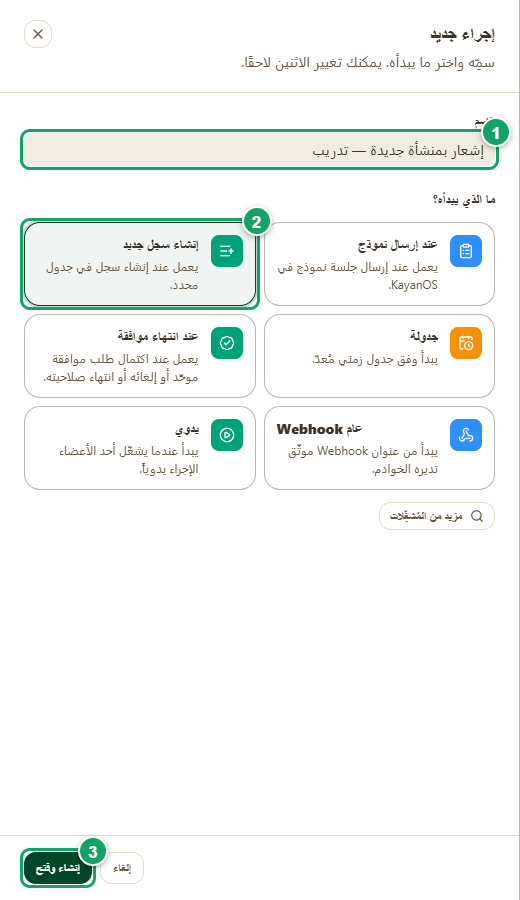
\includegraphics[width=0.55\linewidth]{assets/screens/s1-new-sop.png}
\caption{لوحة «إجراء جديد»}
\label{fig:new-sop}
\shotnote{تطلب اللوحة أمرين فقط: اسماً، وحدثاً يبدأ الإجراء. يبقى زر الإنشاء غير متاح حتى تختار الحدث، لأن الإجراء لا يُبنى دون مشغّل. ① «الاسم»: اكتب اسماً يصف ما يفعله الإجراء. ② «إنشاء سجل جديد»: يبدأ الإجراء كلما أُضيف سجل في جدول تختاره بعد قليل. ③ «إنشاء وفتح».}
\end{figure}
\textbf{تحقق:} يفتح المحرر، وفيه خطوتان جاهزتان: «إنشاء سجل جديد» وتحتها «إنهاء». في رأس الصفحة «لم يُنشر بعد»، وبجانبه شارة صفراء «1 للإصلاح»؛ سنصلحها في الخطوة التالية.

\section{المرحلة 1: أخبر المشغّل أي جدول يراقب}
\label{sec:trigger}
\textbf{لماذا؟} «إنشاء سجل جديد» وحده لا يعرف أي نوع من السجلات تقصد. لهذا تحمل الخطوة الشارة «يحتاج إلى تهيئة»، ولن تستطيع النشر قبل اختيار الجدول.
\begin{enumerate}
\item على اللوحة اضغط بطاقة الخطوة 1، المكتوب تحتها «عند: إنشاء سجل جديد». تفتح لوحة إعدادها على الجانب.
\item اضغط خانة «الجدول»، واكتب جزءاً من الاسم، مثل «المنشآت»، ثم اختر «المنشآت التجارية».
\item لا تضغط «حفظ»؛ لا يوجد زر حفظ. التغييرات تُحفظ وحدها، وتقرأ في رأس المحرر «محفوظ».
\end{enumerate}

\begin{figure}[H]
\centering
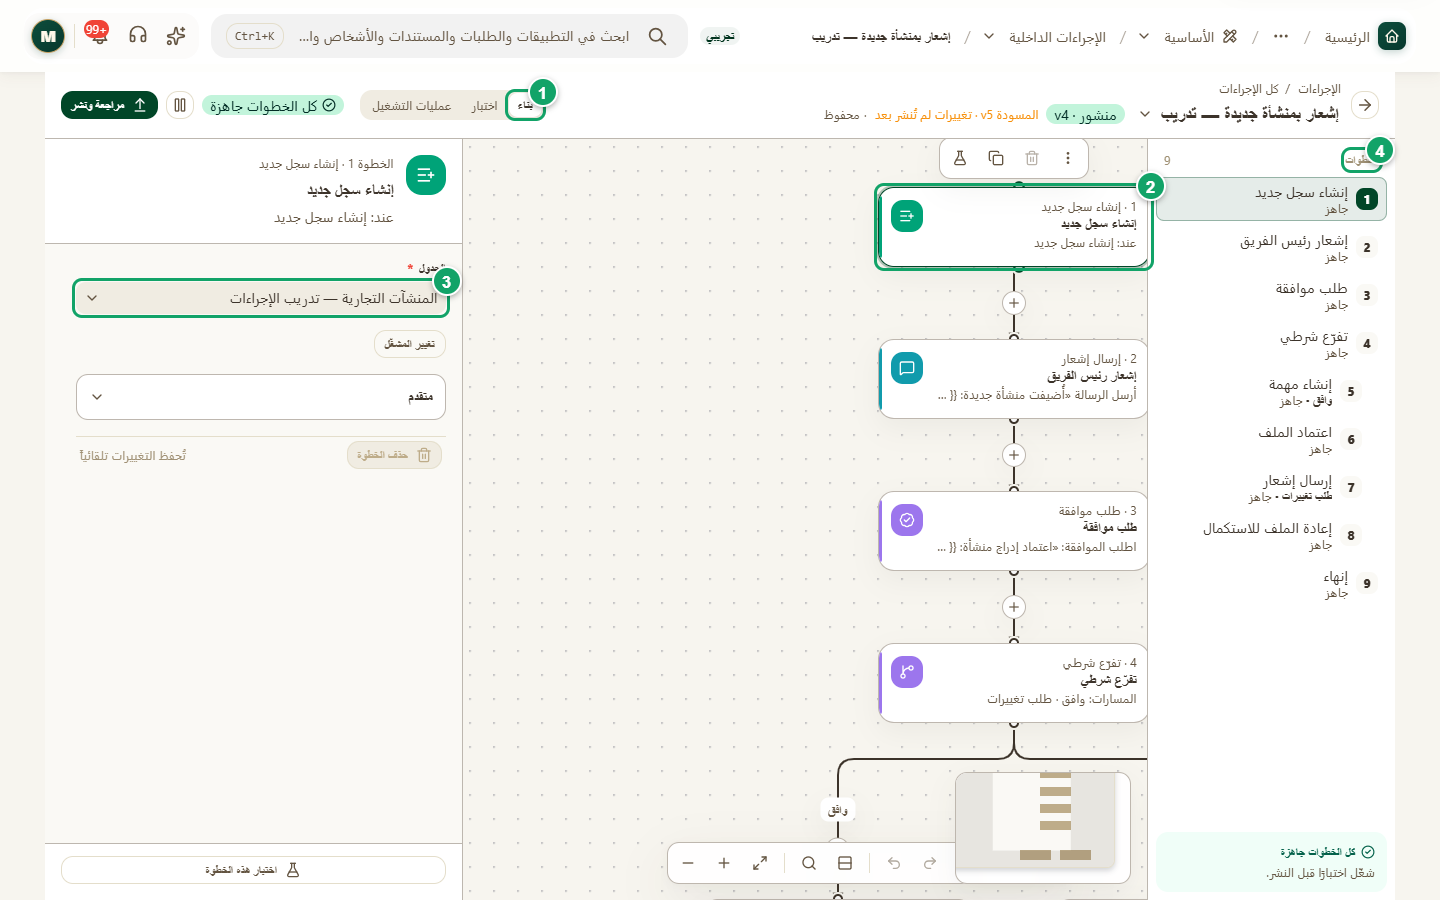
\includegraphics[width=0.95\linewidth]{assets/screens/s1-trigger.png}
\caption{إعداد المشغّل}
\label{fig:trigger}
\shotnote{الصورة من الإجراء نفسه بعد اكتمال المراحل الأربع، لذلك ترى تحته خطوات لم نضفها بعد؛ ركّز الآن على الخطوة 1 فقط. اختيار الجدول هو كل ما يحتاجه هذا المشغّل. ① «بناء»: الوضع الذي تعدّل فيه الخطوات. ② بطاقة المشغّل: اضغطها لتفتح إعدادها. ③ «الجدول»: اختر «المنشآت التجارية». ④ «الخطوات»: قائمة مرقمة تبيّن حالة كل خطوة، مثل «جاهز».}
\end{figure}
\textbf{تحقق:} تحت الخطوة 1 في قائمة «الخطوات» كلمة «جاهز»، وتغيّرت الشارة الصفراء في الرأس إلى «كل الخطوات جاهزة».

\section{المرحلة 1: أضف إشعاراً إلى أحمد}
\label{sec:notify}
\textbf{لماذا؟} هذه أول خطوة تعمل شيئاً يراه أحد. نكتب الآن نصاً ثابتاً، وفي المرحلة الثانية نضيف إليه اسم المنشأة.
\begin{enumerate}
\item على الخط بين الخطوة 1 و«إنهاء» زر صغير «+». اضغطه.
\item تفتح نافذة الخطوات. اكتب في البحث «إرسال إشعار»، ثم اضغط النتيجة «إرسال إشعار». تظهر الخطوة على اللوحة وتفتح لوحة إعدادها.
\item في «عنوان الرسالة» اكتب: «أُضيفت منشأة جديدة».
\item في «محتوى الرسالة» اكتب: «افتح المنشآت التجارية لترى الملف الجديد وراجعه.»
\item اضغط خانة «المستلمون»، واكتب اسم أحمد (أو اسمك وأنت تتدرب)، ثم اختره من القائمة. اضغط \en{Esc} لإغلاق القائمة.
\item اترك بقية الحقول كما هي: «الأولوية» «عادية»، والبقية فارغة.
\end{enumerate}

\begin{figure}[H]
\centering
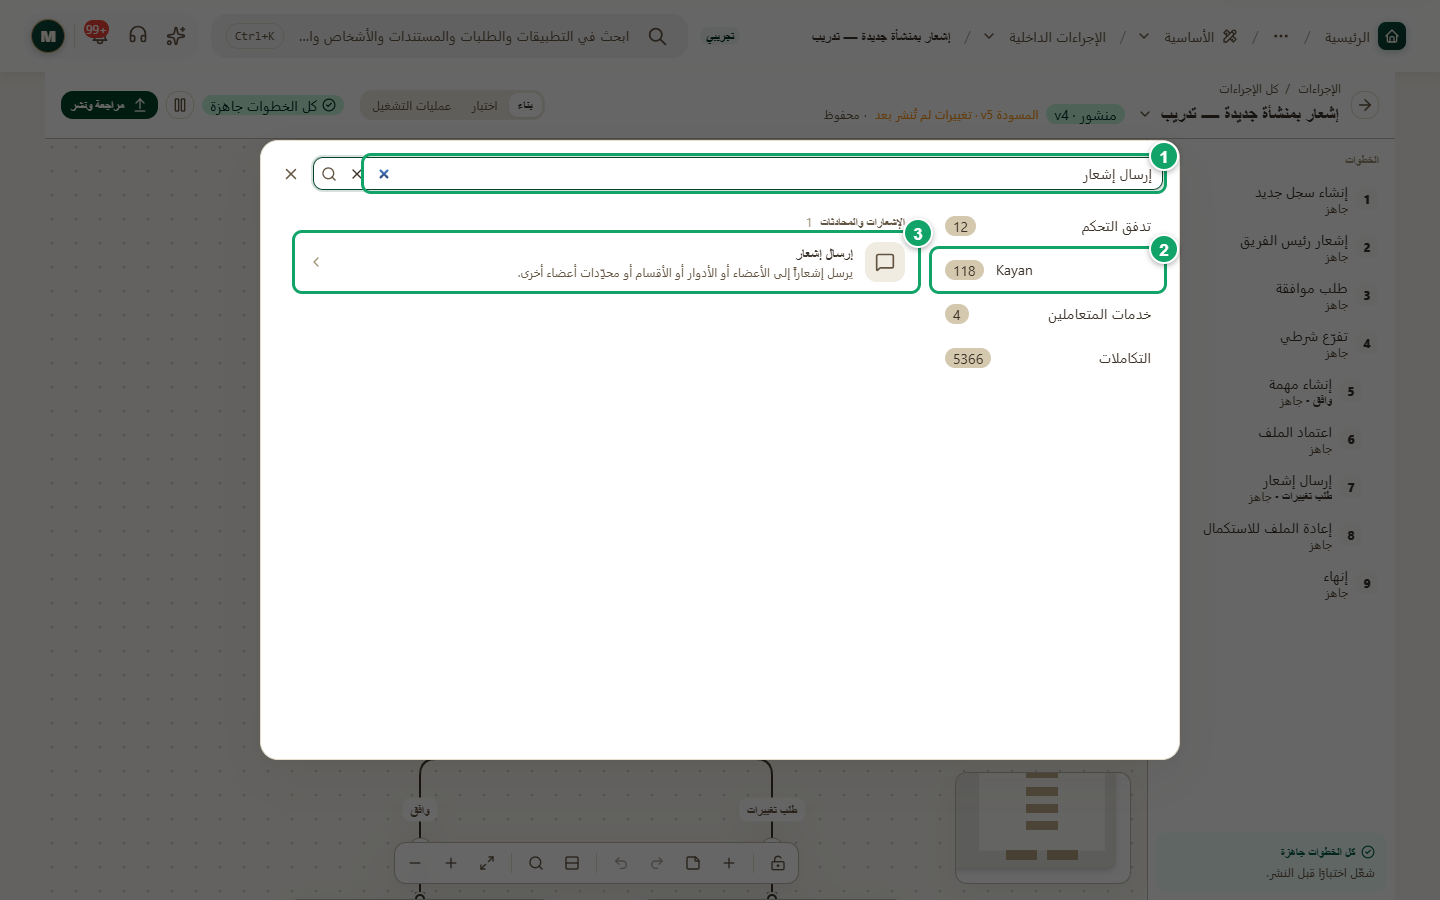
\includegraphics[width=0.95\linewidth]{assets/screens/s1-add-step.png}
\caption{البحث عن خطوة بالاسم}
\label{fig:add-step}
\shotnote{في النافذة مئات الخطوات موزعة على أربع فئات، والبحث بالاسم أسرع طريق إليها. الخطوات التي تعمل داخل كيان، مثل الإشعار والموافقة والسجلات، كلها في فئة «Kayan». ① خانة البحث: اكتب اسم الخطوة. ② «Kayan»: فئة خطوات النظام. ③ «إرسال إشعار»: اضغطها لتضيفها.}
\end{figure}

\begin{figure}[H]
\centering
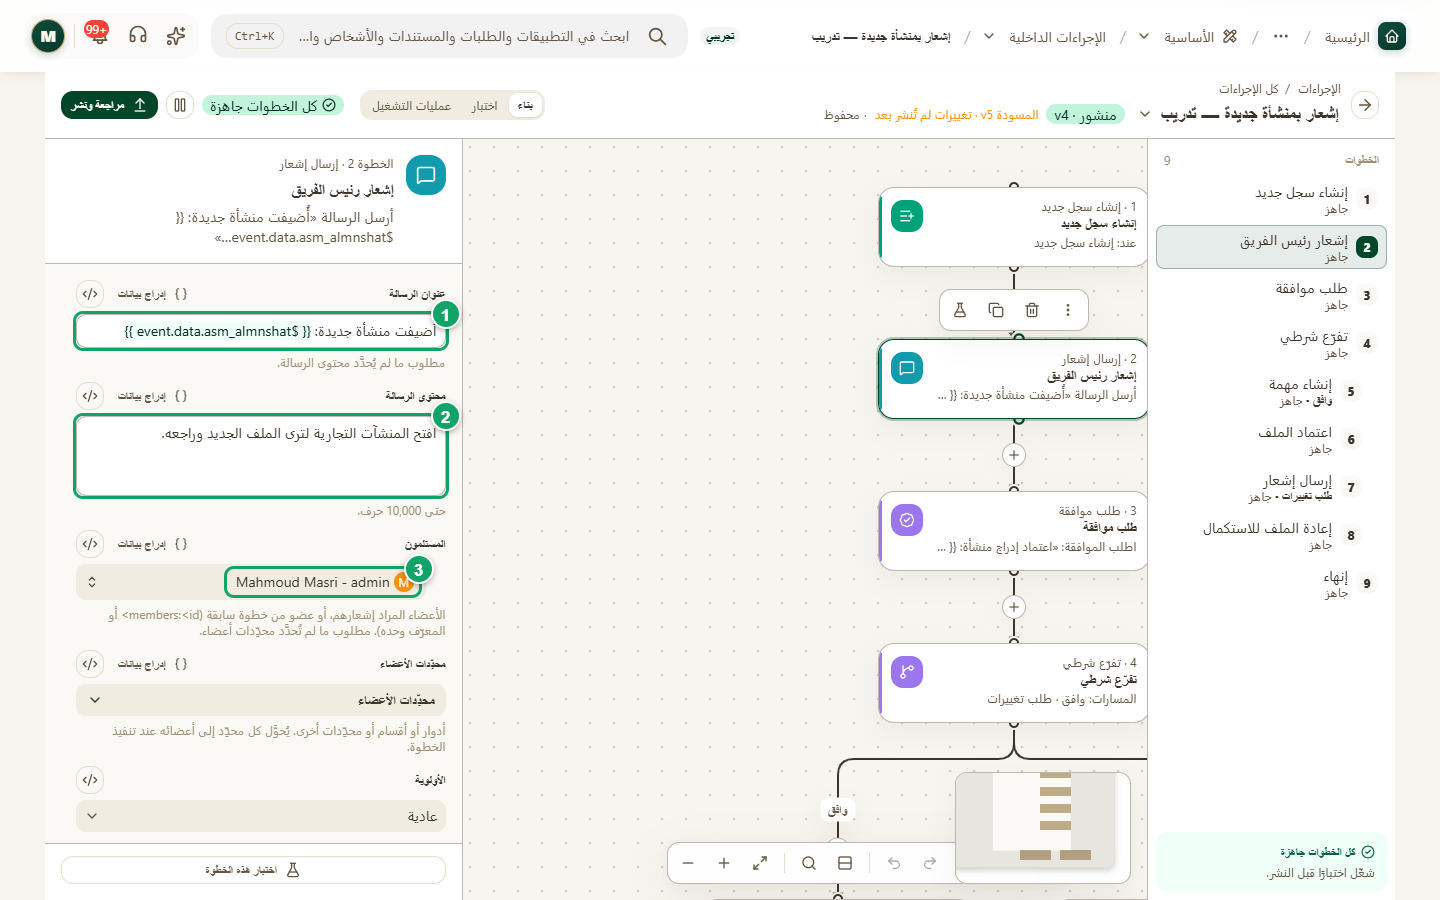
\includegraphics[width=0.95\linewidth]{assets/screens/s1-notify.png}
\caption{حقول «إرسال إشعار»}
\label{fig:notify}
\shotnote{الصورة بعد المرحلة الثانية، لذلك يظهر في العنوان اسم المنشأة مُدرجاً؛ في المرحلة الأولى تكتب العنوان نصاً ثابتاً فقط. ويظهر الحساب المختار في «المستلمون» باسمه، لأن الإشعار يصل إلى عضو محدد. ① «عنوان الرسالة». ② «محتوى الرسالة». ③ «المستلمون»: العضو الذي يصله الإشعار.}
\end{figure}
\textbf{تحقق:} على اللوحة ثلاث بطاقات: «إنشاء سجل جديد» ثم «إرسال إشعار» ثم «إنهاء»، والرأس يقول «كل الخطوات جاهزة».

\section{المرحلة 1: انشر الإصدار الأول}
\label{sec:publish}
\textbf{لماذا؟} كل ما بنيته حتى الآن «مسودة»؛ أي نسخة عمل لا يراها أحد. النشر يحوّلها إلى إصدار يعمل، رقمه \en{v1}.
\begin{enumerate}
\item اضغط «مراجعة ونشر» في رأس المحرر. تفتح لوحة المراجعة.
\item اقرأ «الفحوصات». يجب أن ترى «كل الخطوات مهيّأة.» إن ظهرت مشكلة، فاضغطها وأصلح الخطوة التي تشير إليها.
\item اضغط «نشر \en{v1}» أسفل اللوحة. يمكنك النشر دون اختبار؛ سنجرّب الإجراء بمنشأة حقيقية.
\end{enumerate}

\begin{figure}[H]
\centering
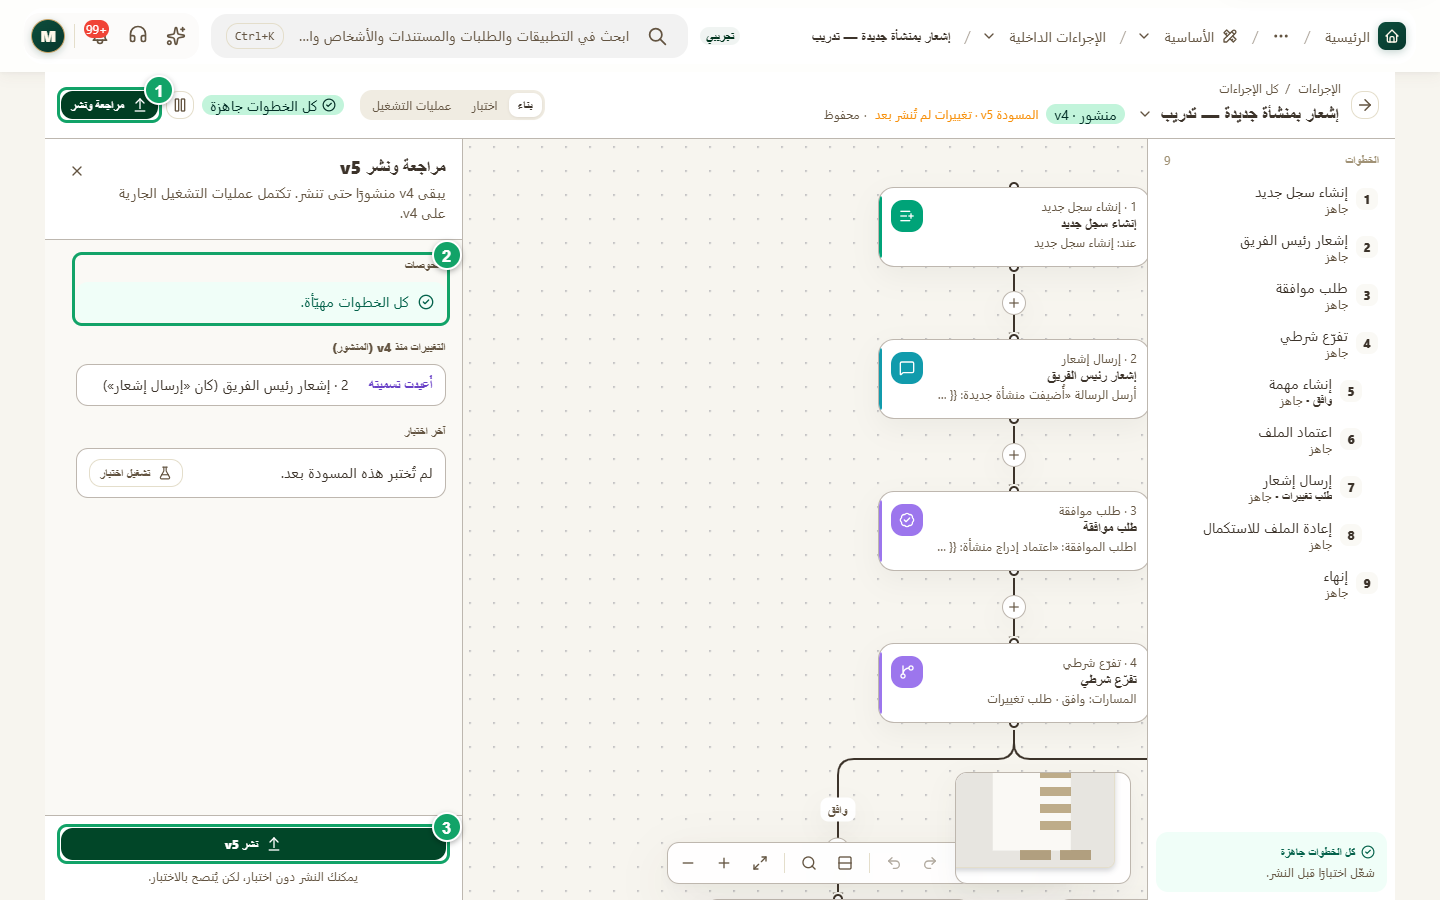
\includegraphics[width=0.95\linewidth]{assets/screens/s1-publish.png}
\caption{لوحة «مراجعة ونشر»}
\label{fig:publish}
\shotnote{تجمع اللوحة ما يجب أن تعرفه قبل النشر: هل كل خطوة مكتملة، وما الذي تغيّر منذ آخر نشر. في الصورة الزر «نشر \en{v5}» لأنها التقطت بعد أربعة إصدارات؛ في أول مرة يكون الزر «نشر \en{v1}». ① «مراجعة ونشر». ② «الفحوصات»: «كل الخطوات مهيّأة.» تعني أن لا شيء يمنع النشر. ③ زر النشر.}
\end{figure}
\textbf{تحقق:} تظهر رسالة «أصبح \en{v1} منشورًا»، ويتغير الرأس إلى «منشور · \en{v1}» ثم «لا توجد تغييرات غير منشورة».

\section{المرحلة 1: أضف منشأة وشاهد الإجراء يعمل}
\label{sec:first-run}
\textbf{لماذا؟} هذا هو الاختبار الحقيقي: يعمل نور كعادته، ولا يعرف أن هناك إجراءً، والإجراء يعمل خلفه.
\begin{enumerate}
\item افتح «المنشآت التجارية» من قائمة تطبيقك، ثم اضغط «إضافة».
\item في «اسم المنشأة» اكتب «فرن السنابل — تدريب».
\item في «حالة الملف» اضغط «بانتظار الاعتماد».
\item اضغط «إنشاء».
\end{enumerate}

\begin{figure}[H]
\centering
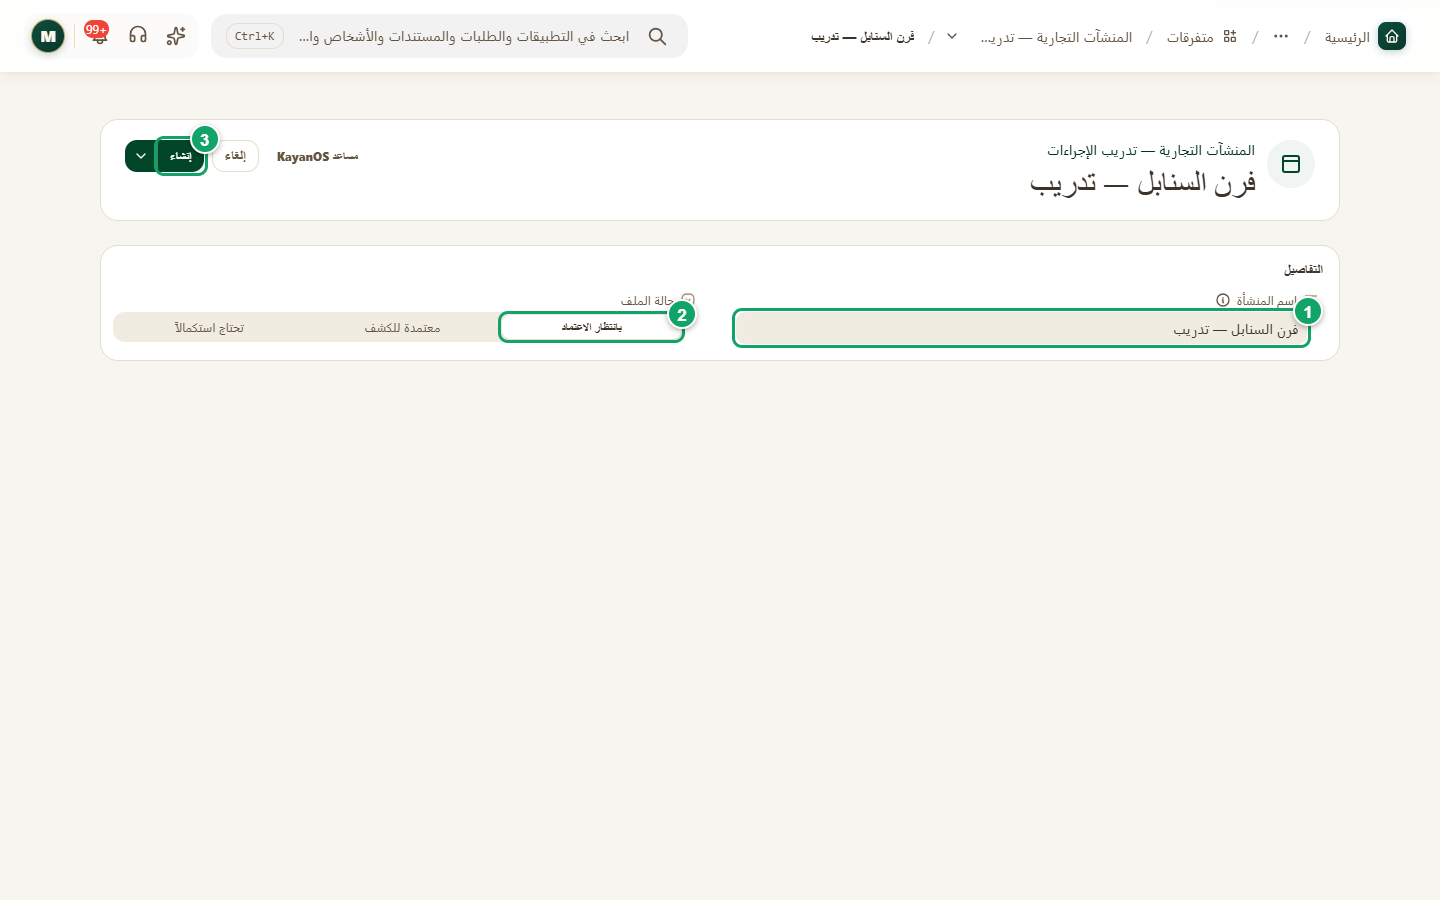
\includegraphics[width=0.95\linewidth]{assets/screens/s1-add-record.png}
\caption{إضافة منشأة}
\label{fig:add-record}
\shotnote{هذه شاشة الإضافة العادية التي يستخدمها نور كل يوم، ولا شيء فيها يدل على الإجراء. إنشاء السجل هو الحدث الذي ينتظره المشغّل. ① «اسم المنشأة». ② «بانتظار الاعتماد»: حالة كل ملف جديد. ③ «إنشاء»: لحظة الضغط عليه يبدأ الإجراء.}
\end{figure}
\begin{rcnote}[اسم جديد لكل تجربة]
في كل مرة تجرّب فيها الإجراء، أضف منشأة باسم جديد، مثل «مخبز الريحان — تدريب» ثم «فرن القمح — تدريب». هكذا تميّز كل عملية تشغيل وكل إشعار عن غيره.
\end{rcnote}
\textbf{تحقق:} تعود إلى قائمة «المنشآت التجارية»، وفيها «فرن السنابل — تدريب» بحالة «بانتظار الاعتماد».

\section{المرحلة 1: اقرأ ما حدث، ثم افتح الإشعار}
\label{sec:read-run}
\textbf{لماذا؟} يجب أن تعرف من مكانين أن الإجراء عمل: من عملية التشغيل في المحرر، ومن الإشعار الذي وصل فعلاً.
\begin{enumerate}
\item ارجع إلى الإجراء، واضغط «عمليات التشغيل» في رأس المحرر.
\item في القائمة عملية تشغيل حالتها «مكتمل». اضغطها.
\item انظر إلى اللوحة: على كل خطوة كلمة «نجح». وتحت «التشغيل المحدد» عدد الخطوات الناجحة.
\item اضغط جرس «الإشعارات» أعلى الصفحة، ثم تبويب «المستجدات».
\end{enumerate}

\begin{figure}[H]
\centering
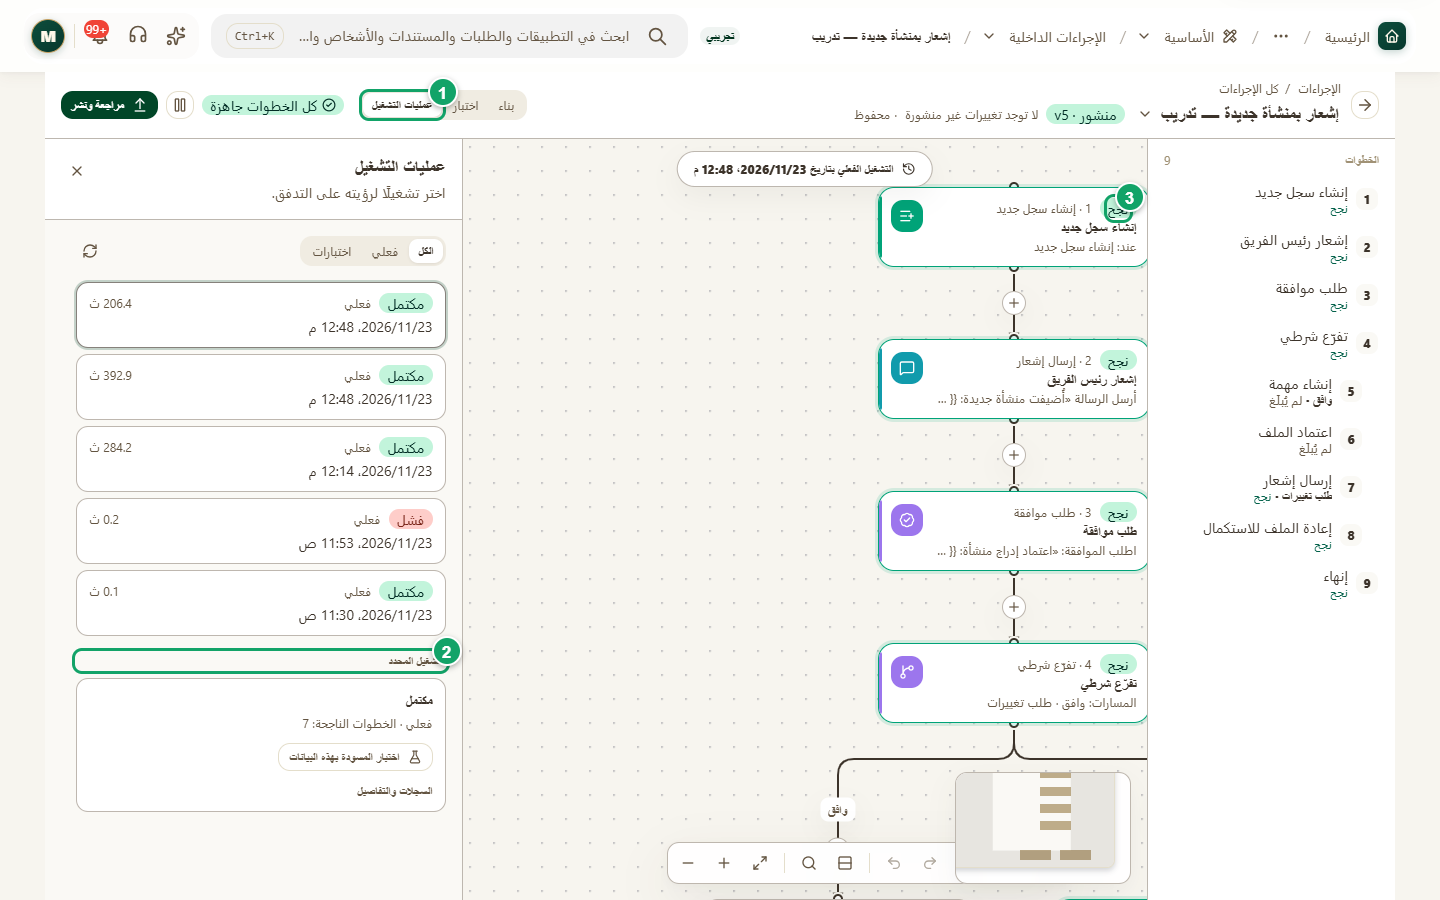
\includegraphics[width=0.95\linewidth]{assets/screens/s1-runs.png}
\caption{عملية تشغيل مكتملة}
\label{fig:runs}
\shotnote{عند اختيار عملية من القائمة تظهر نتيجتها على اللوحة نفسها، خطوة خطوة. الصورة من تشغيل في المرحلة الرابعة، لذلك فيه خطوات أكثر؛ في المرحلة الأولى ترى ثلاث خطوات فقط. ① «عمليات التشغيل». ② «التشغيل المحدد»: حالة العملية وعدد خطواتها الناجحة. ③ «نجح»: نتيجة الخطوة في هذه العملية.}
\end{figure}

\begin{figure}[H]
\centering
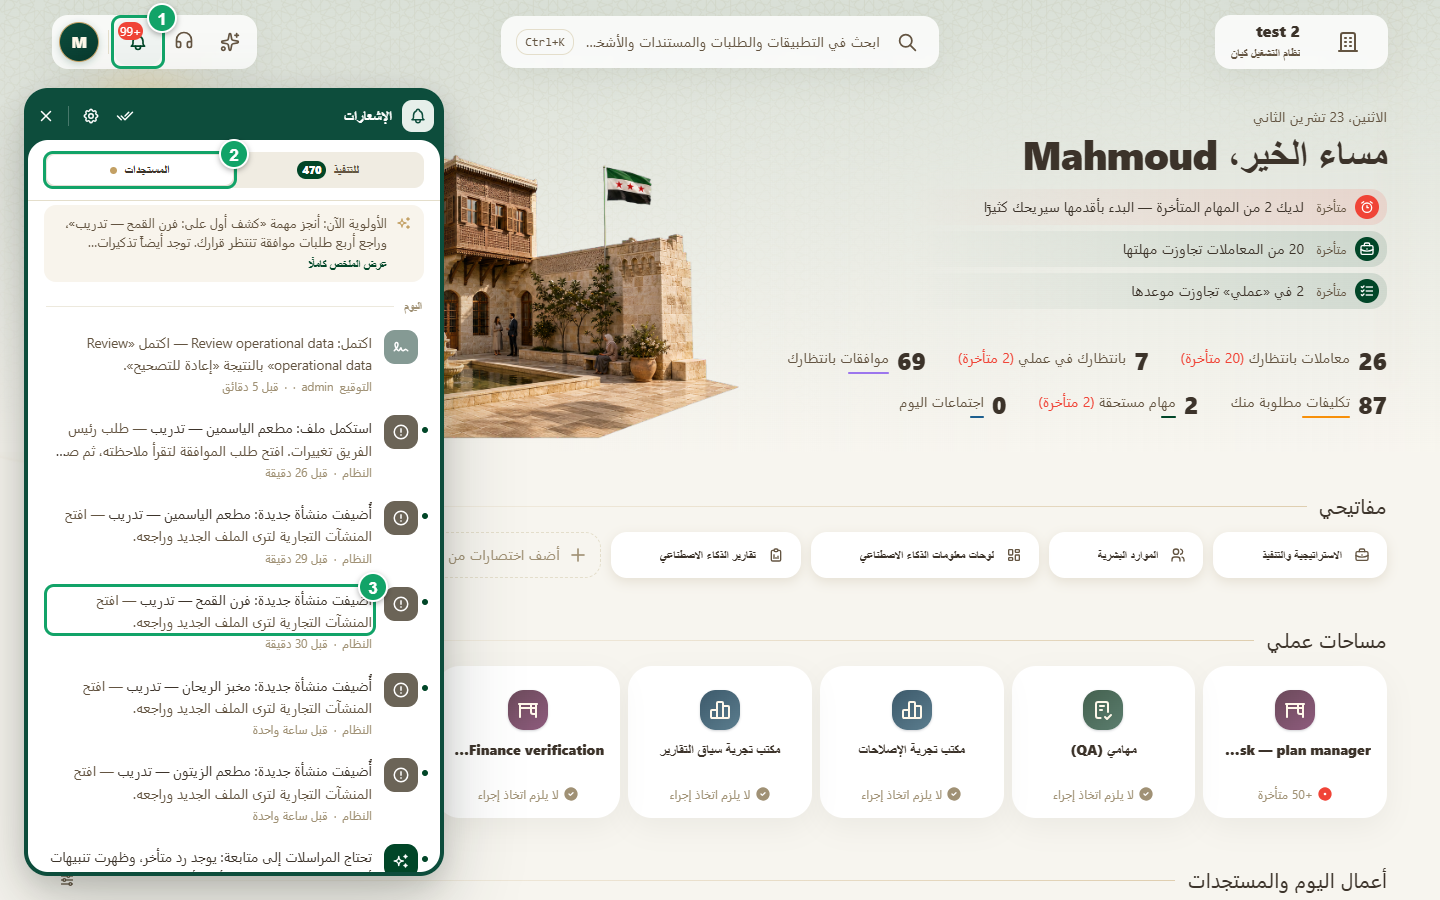
\includegraphics[width=0.95\linewidth]{assets/screens/s1-notification.png}
\caption{الإشعار في «المستجدات»}
\label{fig:notification}
\shotnote{إشعارات الإجراء تظهر في تبويب «المستجدات»، لا في «للتنفيذ» المفتوح أولاً. لذلك إذا فتحت الجرس ولم تجد الإشعار، فانتقل إلى التبويب الثاني قبل أن تظن أن الإجراء لم يعمل. ① جرس «الإشعارات». ② «المستجدات». ③ الإشعار: عنوانه ومحتواه كما كتبتهما في الخطوة.}
\end{figure}
\textbf{تحقق:} في «المستجدات» إشعار «أُضيفت منشأة جديدة». أنهيت المرحلة الأولى: لديك إجراء منشور يعمل.

\section{المرحلة 2: أضف اسم المنشأة إلى الإشعار}
\label{sec:insert-data}
\textbf{لماذا؟} «أُضيفت منشأة جديدة» لا يقول أي منشأة. نريد أن يكون العنوان «أُضيفت منشأة جديدة: فرن السنابل — تدريب»، ويتغير الاسم وحده مع كل منشأة. لا نكتب الاسم بأيدينا، بل «ندرجه» من بيانات المشغّل.
\begin{enumerate}
\item ارجع إلى وضع «بناء»، واضغط خطوة «إرسال إشعار».
\item في «عنوان الرسالة» ضع المؤشر بعد آخر كلمة، واكتب «: » (نقطتان ثم مسافة).
\item اضغط «إدراج بيانات» فوق الحقل. تفتح قائمة صغيرة.
\item في «ابحث في الحقول» اكتب اسم منشأة أضفتها، مثل «فرن». تظهر الحقول التي فيها هذه القيمة.
\item اضغط السطر الذي يبدأ بـ\en{data.} ويحمل اسم المنشأة. في مثالنا \en{data.asm\_almnshat}.
\end{enumerate}

\begin{figure}[H]
\centering
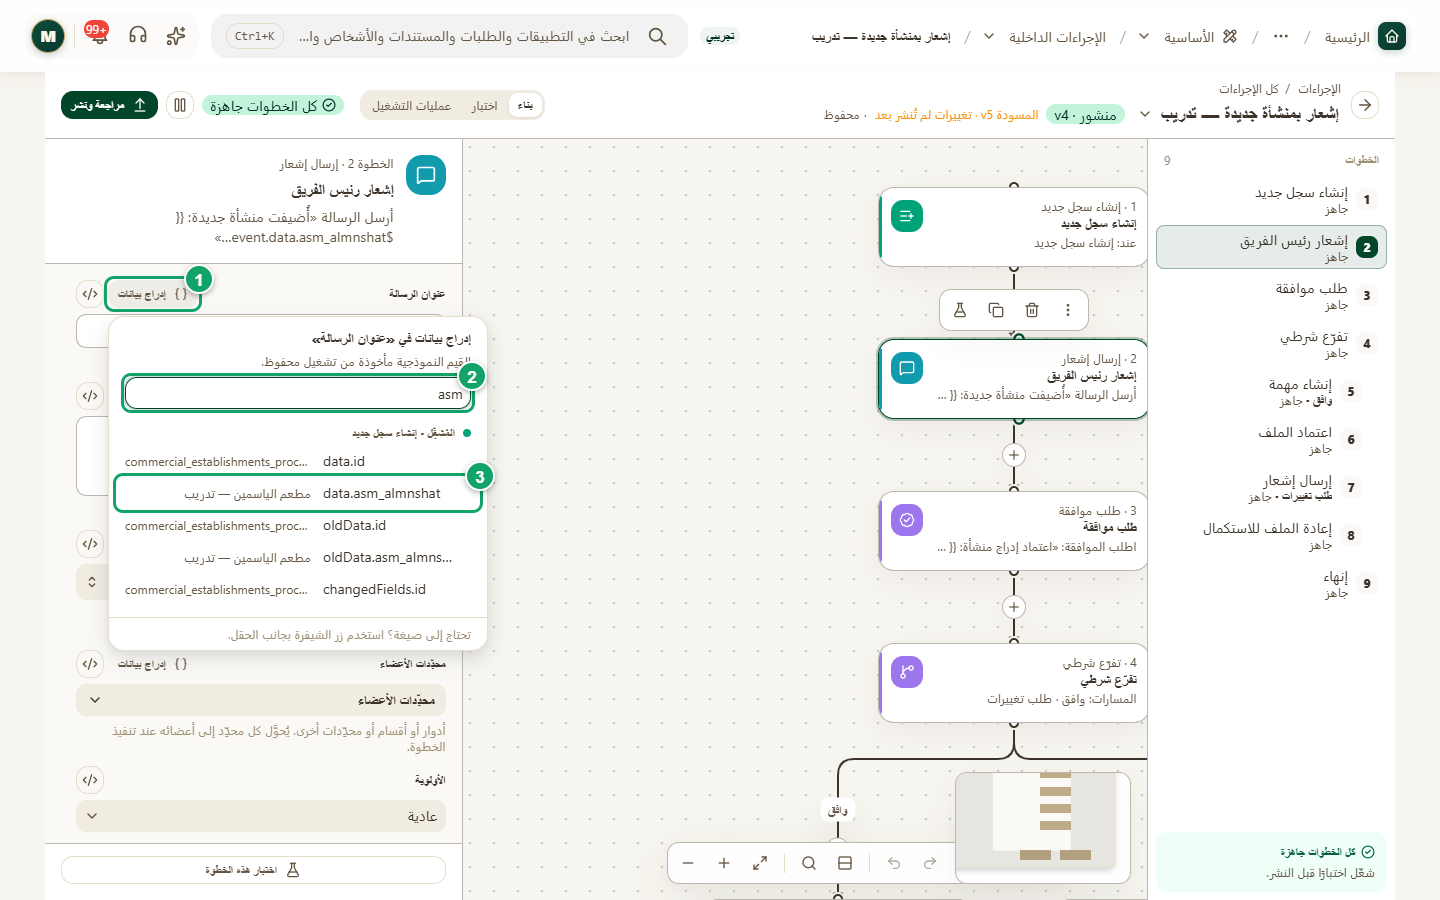
\includegraphics[width=0.95\linewidth]{assets/screens/s2-insert-data.png}
\caption{إدراج اسم المنشأة من بيانات المشغّل}
\label{fig:insert-data}
\shotnote{تعرض القائمة حقول آخر عملية تشغيل مع قيمها، فتعرف الحقل من قيمته لا من اسمه. اسم الحقل إنجليزي ولّده النظام من عنوانه العربي، لذلك البحث بالقيمة أسهل. ① «إدراج بيانات». ② «ابحث في الحقول»: اكتب اسم منشأة، أو \en{asm}. ③ \en{data.asm\_almnshat}: الاسم في السجل الجديد؛ اضغطه.}
\end{figure}

\begin{rcnote}[لماذا جرّبنا قبل الإدراج؟]
قبل أول عملية تشغيل تعرض القائمة حقولاً من مثال عام لا يخص جدولك. بعد أن أضفت «فرن السنابل — تدريب» صارت تعرض حقولك الحقيقية وقيمها. هذا سبب ترتيب المراحل: جرّب أولاً، ثم أدرج البيانات.
\end{rcnote}
\textbf{تحقق:} يصبح العنوان «أُضيفت منشأة جديدة: \en{\{\{ \$event.data.asm\_almnshat \}\}}». هذا الرمز بين القوسين المزدوجين يعني «اسم المنشأة»، وسيُستبدل بالاسم الحقيقي عند التشغيل. في الرأس الآن «المسودة \en{v2} · تغييرات لم تُنشر بعد».

\section{المرحلة 2: أضف «طلب موافقة» واكتب عنوانه}
\label{sec:approval}
\textbf{لماذا؟} الإشعار يُعلم أحمد فقط. أما «طلب موافقة» فيطلب منه قراراً، ويوقف الإجراء حتى يرد. وبعد الرد يحفظ النظام ما اختاره أحمد.
\begin{enumerate}
\item اضغط «+» على الخط بين «إرسال إشعار» و«إنهاء».
\item اكتب في البحث «طلب موافقة»، ثم اختر «طلب موافقة».
\item في «عنوان الموافقة» اكتب «اعتماد إدراج منشأة: »، ثم اضغط «إدراج بيانات» وأدرج اسم المنشأة كما في الخطوة السابقة.
\item في «تفاصيل الموافقة» اكتب: «راجع ملف المنشأة. وافق إذا كانت البيانات مكتملة، أو اطلب تغييرات واكتب الناقص.»
\end{enumerate}

\begin{figure}[H]
\centering
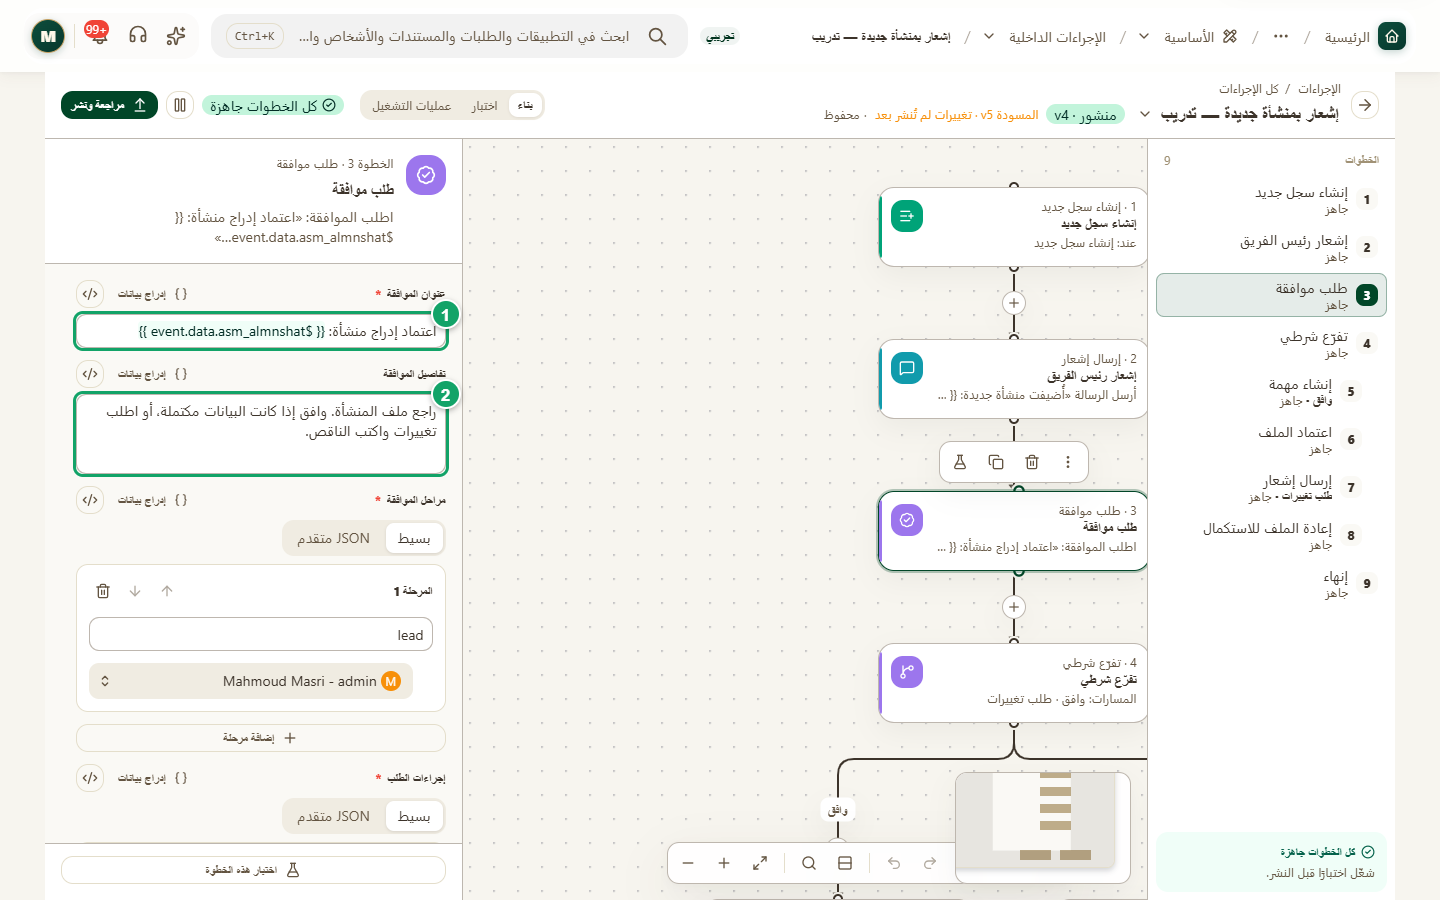
\includegraphics[width=0.95\linewidth]{assets/screens/s2-approval-fields.png}
\caption{عنوان الطلب وتفاصيله}
\label{fig:approval-fields}
\shotnote{العنوان هو ما يراه أحمد في قائمة طلباته، والتفاصيل تخبره بما يراجعه. إدراج اسم المنشأة في العنوان يجعل كل طلب مختلفاً عن غيره في القائمة. ① «عنوان الموافقة»: مطلوب. ② «تفاصيل الموافقة».}
\end{figure}
\textbf{تحقق:} تظهر الخطوة على اللوحة بين الإشعار و«إنهاء»، ويظهر عنوانها تحت اسمها.

\section{المرحلة 2: اختر من يوافق}
\label{sec:approver}
\textbf{لماذا؟} الطلب يمر بـ«مراحل»؛ وكل مرحلة شخص أو أكثر يجب أن يرد. نحتاج مرحلة واحدة فيها أحمد.
\begin{enumerate}
\item انزل في لوحة الإعداد إلى «مراحل الموافقة»، واضغط «إضافة مرحلة».
\item في الخانة الأولى من «المرحلة 1» (يظهر فيها «مدير» رمادياً) اكتب \en{lead}. هذا مفتاح إنجليزي قصير للمرحلة، ولا يراه أحمد.
\item اضغط «تحديد» تحتها، واكتب اسم أحمد (أو اسمك)، ثم اختره. اضغط \en{Esc}.
\end{enumerate}

\begin{figure}[H]
\centering
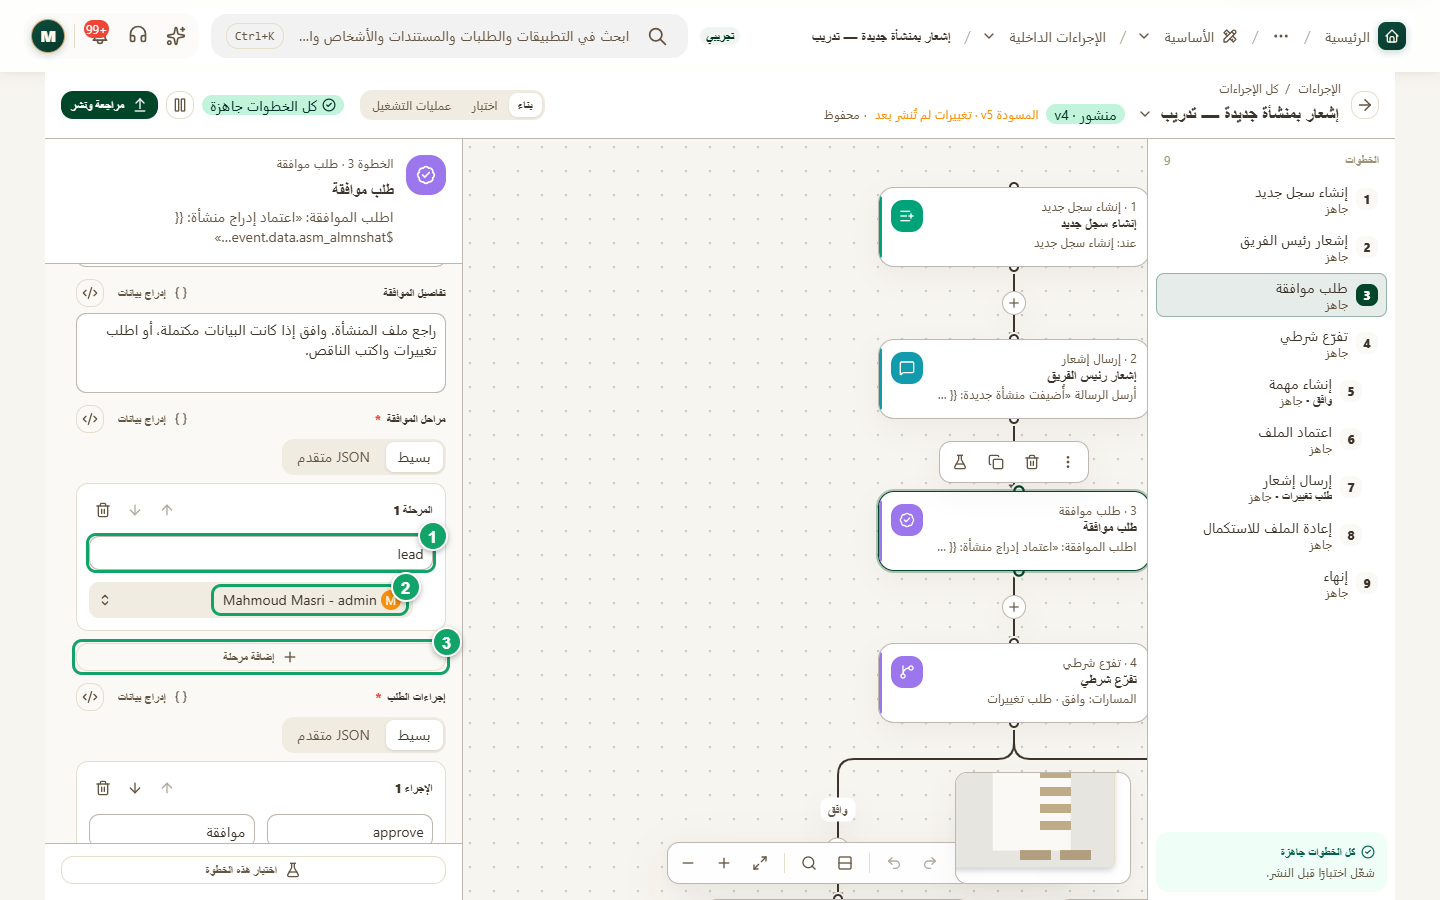
\includegraphics[width=0.95\linewidth]{assets/screens/s2-approval-stage.png}
\caption{مرحلة الموافقة الوحيدة}
\label{fig:approver}
\shotnote{تحتاج كل مرحلة مفتاحاً ومعتمداً واحداً على الأقل، وإلا ظهرت تحتها رسالة حمراء ولم تصبح الخطوة جاهزة. نكتفي بمرحلة واحدة؛ «إضافة مرحلة» تضيف مستوى اعتماد آخر بعدها. ① مفتاح المرحلة: \en{lead}. ② المعتمد. ③ «إضافة مرحلة».}
\end{figure}
\textbf{تحقق:} اختفت الرسالتان الحمراوان «مفتاح المرحلة مطلوب» و«مطلوب معتمد واحد على الأقل».

\section{المرحلة 2: اكتب أزرار الرد بالعربية}
\label{sec:actions}
\textbf{لماذا؟} تحت «إجراءات الطلب» زرّان جاهزان يراهما أحمد عندما يرد، لكن تسميتهما بالإنجليزية: \en{Approve} و\en{Request changes}. سنكتبهما بالعربية، ونلغي طلب التوقيع حتى يكون الرد ضغطة واحدة.
\begin{enumerate}
\item انزل إلى «إجراءات الطلب». في «الإجراء 1» ثلاث خانات: المفتاح \en{approve}، والتسمية، والنتيجة \en{approved}. غيّر التسمية \en{Approve} إلى «موافقة».
\item تحت «التوقيع» في «الإجراء 1» اضغط «لا شيء».
\item في «الإجراء 2» غيّر التسمية \en{Request changes} إلى «طلب تغييرات». اترك «التعليق» «مطلوب»؛ يجب أن يكتب أحمد ما الناقص.
\item لا تغيّر المفاتيح ولا النتائج. سنقرأ النتيجتين \en{approved} و\en{needs\_changes} في المرحلة الثالثة.
\end{enumerate}

\begin{figure}[H]
\centering
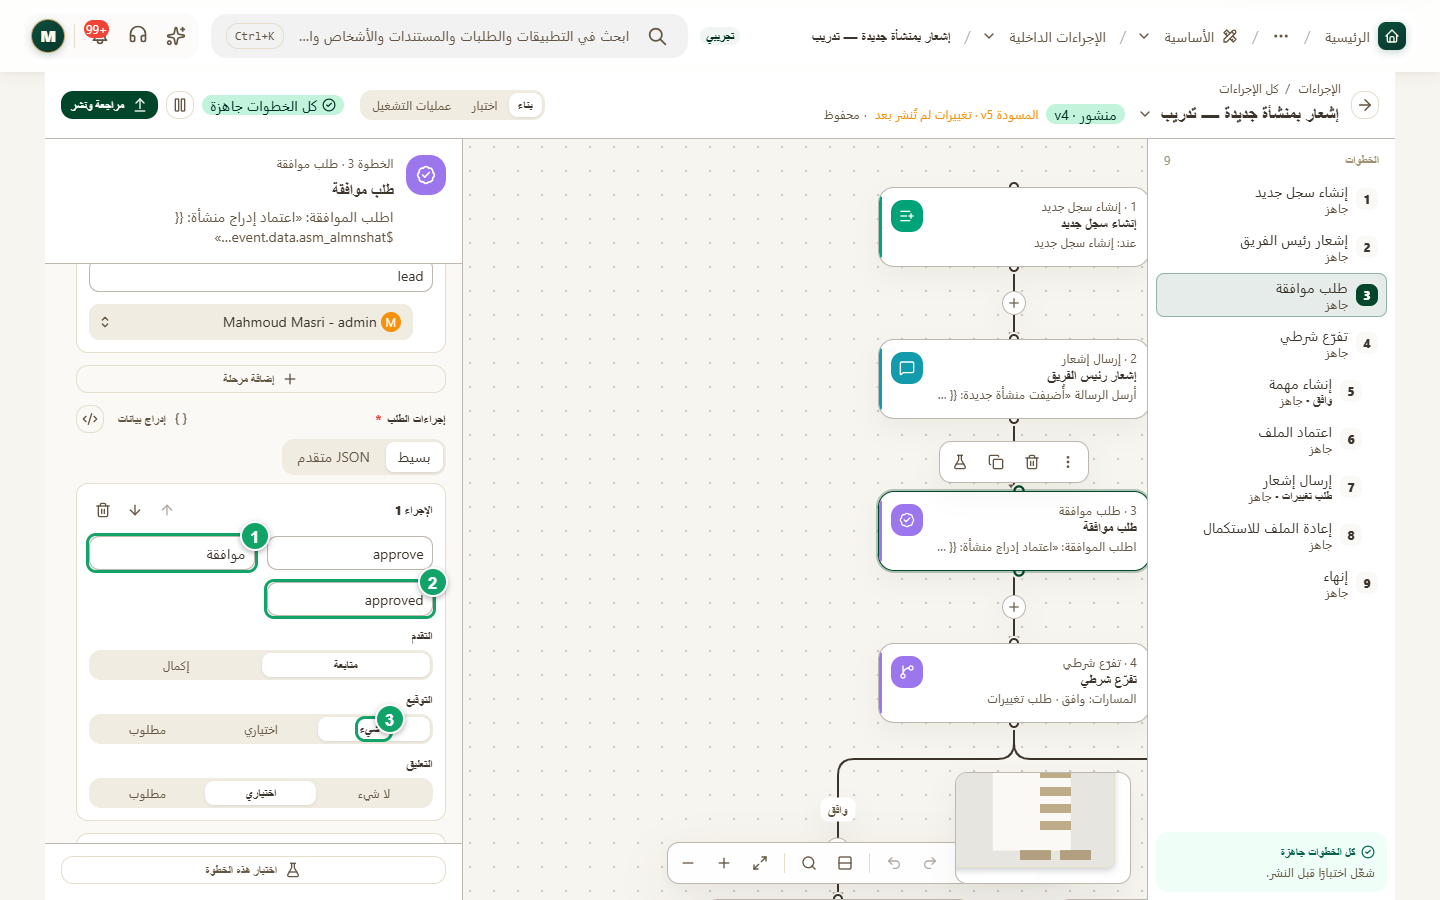
\includegraphics[width=0.95\linewidth]{assets/screens/s2-approval-actions.png}
\caption{تسمية أول زر رد ونتيجته}
\label{fig:actions}
\shotnote{لكل زر ثلاثة أشياء: ما يراه أحمد، وما يحفظه النظام، وما يُطلب منه عند الضغط. التسمية للعين فقط، أما النتيجة فهي ما يقرؤه الإجراء بعد الرد، لذلك نغيّر الأولى ونترك الثانية. ① التسمية: «موافقة». ② النتيجة: \en{approved}. ③ «لا شيء» تحت «التوقيع»: الموافقة بلا توقيع.}
\end{figure}
\textbf{تحقق:} في «الإجراء 1» التسمية «موافقة» و«التوقيع» «لا شيء»، وفي «الإجراء 2» التسمية «طلب تغييرات».

\section{المرحلة 2: خطوة ضرورية في «مرفقات المكتبة»}
\label{sec:attachments}
\textbf{لماذا؟} في الإصدار الحالي من كيان، إذا تركت «مرفقات المكتبة» فارغة، يفشل الطلب عند التشغيل برسالة «Internal command failed with status 422»، ولا يصل إلى أحمد. جرّبنا ذلك في بيئة الاختبار، والحل أن نكتب في الخانة قائمة فارغة صراحة.
\begin{enumerate}
\item انزل إلى «مرفقات المكتبة». بجانب عنوانها زر صغير عليه \en{</>}؛ هذا «زر التعبير». اضغطه.
\item تفتح خانة داكنة فيها \en{""}. احذف ما فيها، واكتب القوس \en{[} فقط؛ يضيف المحرر القوس الثاني وحده فتصبح \en{[]}.
\item اضغط \en{Esc}.
\item انزل إلى «المهلة الزمنية» وغيّر \en{30 days} إلى \en{5 days}. هذه المدة التي ينتظر فيها الإجراء رد أحمد.
\end{enumerate}

\begin{figure}[H]
\centering
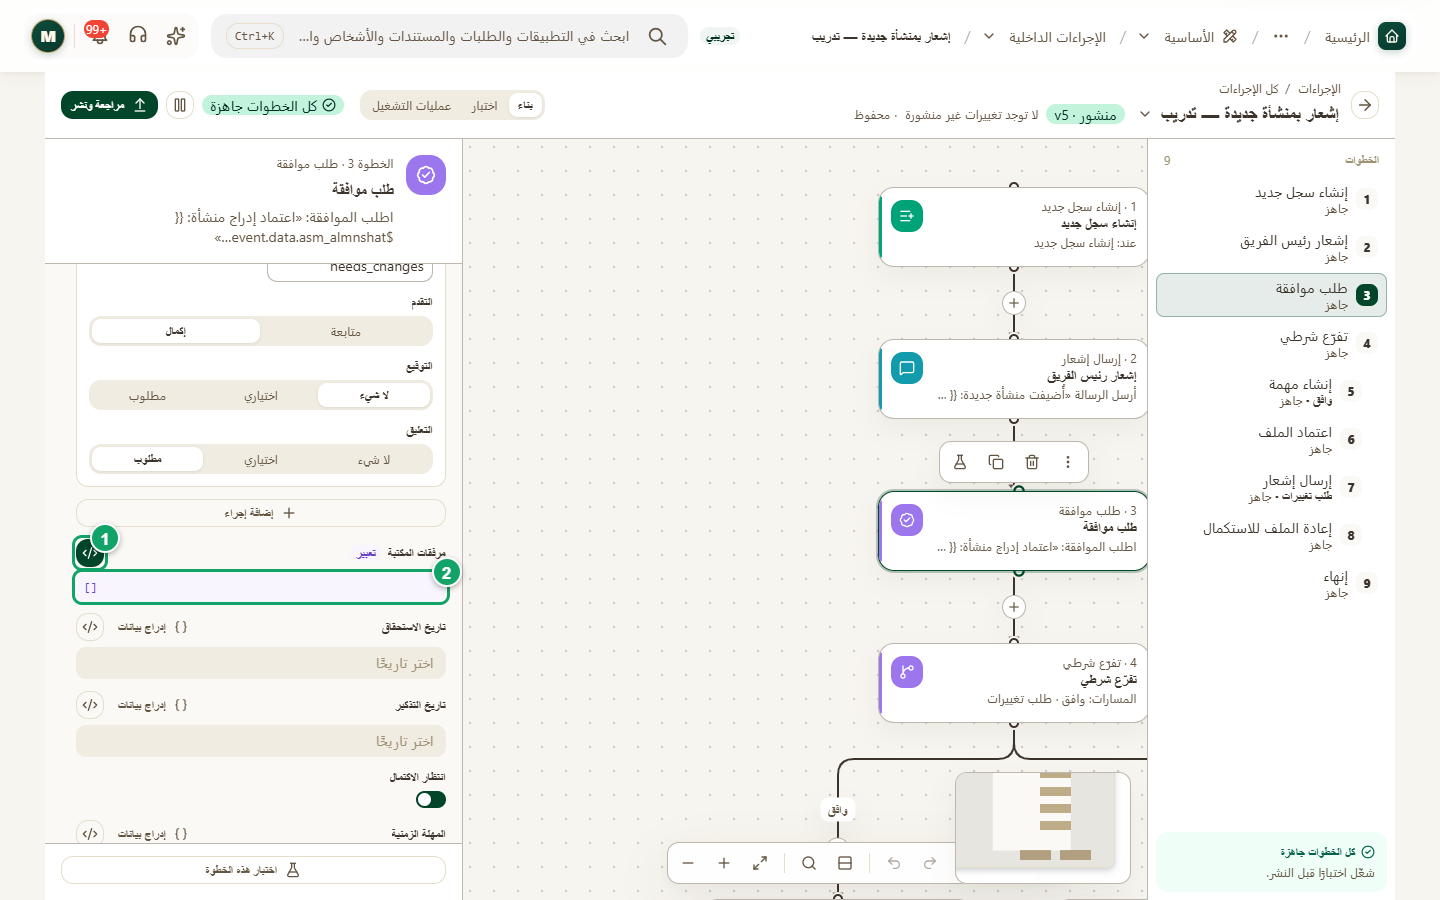
\includegraphics[width=0.95\linewidth]{assets/screens/s2-attachments.png}
\caption{القائمة الفارغة في «مرفقات المكتبة»}
\label{fig:attachments}
\shotnote{بعد الضغط على زر التعبير تتحول الخانة إلى تعبير، ويظهر بجانب عنوانها كلمة «تعبير». القوسان \en{[]} يعنيان «لا مرفقات»، وهذا ما يحتاجه الطلب ليعمل. ① زر التعبير \en{</>}. ② \en{[]}.}
\end{figure}
\begin{rcwarn}[إن نسيت هذه الخطوة]
تظهر العملية في «عمليات التشغيل» بحالة «فشل»، وتحت «التشغيل المحدد»: «فشل عند 3 · طلب موافقة» ثم «Internal command failed with status 422». أضف \en{[]} كما في الخطوات أعلاه، وانشر من جديد، ثم أضف منشأة جديدة.
\end{rcwarn}
\textbf{تحقق:} تحت «مرفقات المكتبة» كلمة «تعبير» والقيمة \en{[]}، و«المهلة الزمنية» \en{5 days}.

\section{المرحلة 2: انشر، ثم دع أحمد يرد}
\label{sec:respond}
\textbf{لماذا؟} الآن يتوقف الإجراء في منتصفه وينتظر إنساناً. سنرى الطلب كما يراه أحمد، ونرد عليه.
\begin{enumerate}
\item اضغط «مراجعة ونشر» ← «نشر \en{v2}».
\item أضف منشأة جديدة: «مخبز الريحان — تدريب» بحالة «بانتظار الاعتماد». تظهر أسفل الشاشة رسالة «يتطلب «اعتماد إدراج منشأة: مخبز الريحان — تدريب» ردك.»
\item بحساب أحمد افتح «طلبات بانتظارك» من القائمة الرئيسية، وابقَ في تبويب «بانتظارك».
\item اضغط بطاقة «اعتماد إدراج منشأة: مخبز الريحان — تدريب». تفتح تفاصيلها.
\item اضغط «موافقة»، ثم «تأكيد موافقة» في النافذة الصغيرة. التعليق اختياري هنا.
\end{enumerate}

\begin{figure}[H]
\centering
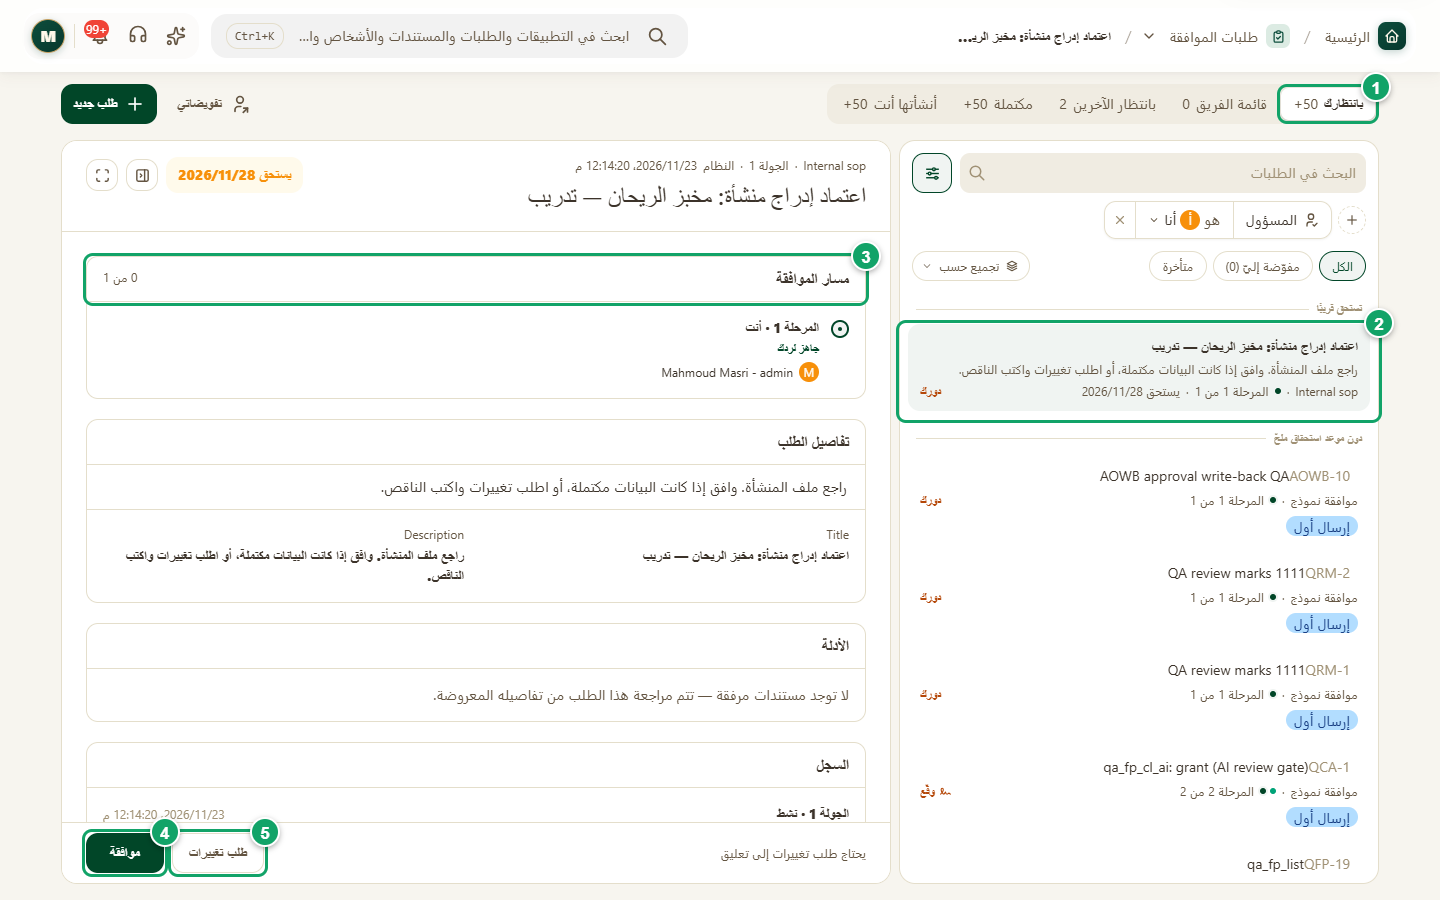
\includegraphics[width=0.95\linewidth]{assets/screens/s2-approval-request.png}
\caption{الطلب كما يراه أحمد}
\label{fig:approval-request}
\shotnote{أحمد لا يرى المحرر ولا الخطوات؛ يرى طلباً بعنوان واضح، وتفاصيل، ومن يجب أن يرد، وزرين بالعربية كما كتبناهما. ① «بانتظارك»: الطلبات التي تنتظر ردك. ② بطاقة الطلب. ③ «مسار الموافقة»: المرحلة الوحيدة، وفيها أحمد. ④ «موافقة». ⑤ «طلب تغييرات»: يطلب تعليقاً قبل التأكيد.}
\end{figure}
\textbf{تحقق:} يخرج الطلب من «بانتظارك». وفي «عمليات التشغيل» صارت العملية «مكتمل» بعد أن كانت تنتظر. أنهيت المرحلة الثانية.

\section{المرحلة 3: أعطِ طلب الموافقة اسماً يقرؤه الإجراء}
\label{sec:reference}
\textbf{لماذا؟} في المرحلة الثالثة سنسأل: «بماذا رد أحمد؟» لنسأل عن نتيجة خطوة، نحتاج اسماً إنجليزياً قصيراً لها اسمه «الاسم المرجعي».
\begin{enumerate}
\item اضغط خطوة «طلب موافقة»، ثم انزل إلى «متقدم» واضغطه ليفتح.
\item اضغط «امنحها اسمًا مقروءًا». تظهر خانة «الاسم المرجعي» وفيها \en{step}.
\item احذف \en{step} واكتب \en{approval}، ثم اضغط \en{Enter}.
\end{enumerate}

\begin{figure}[H]
\centering
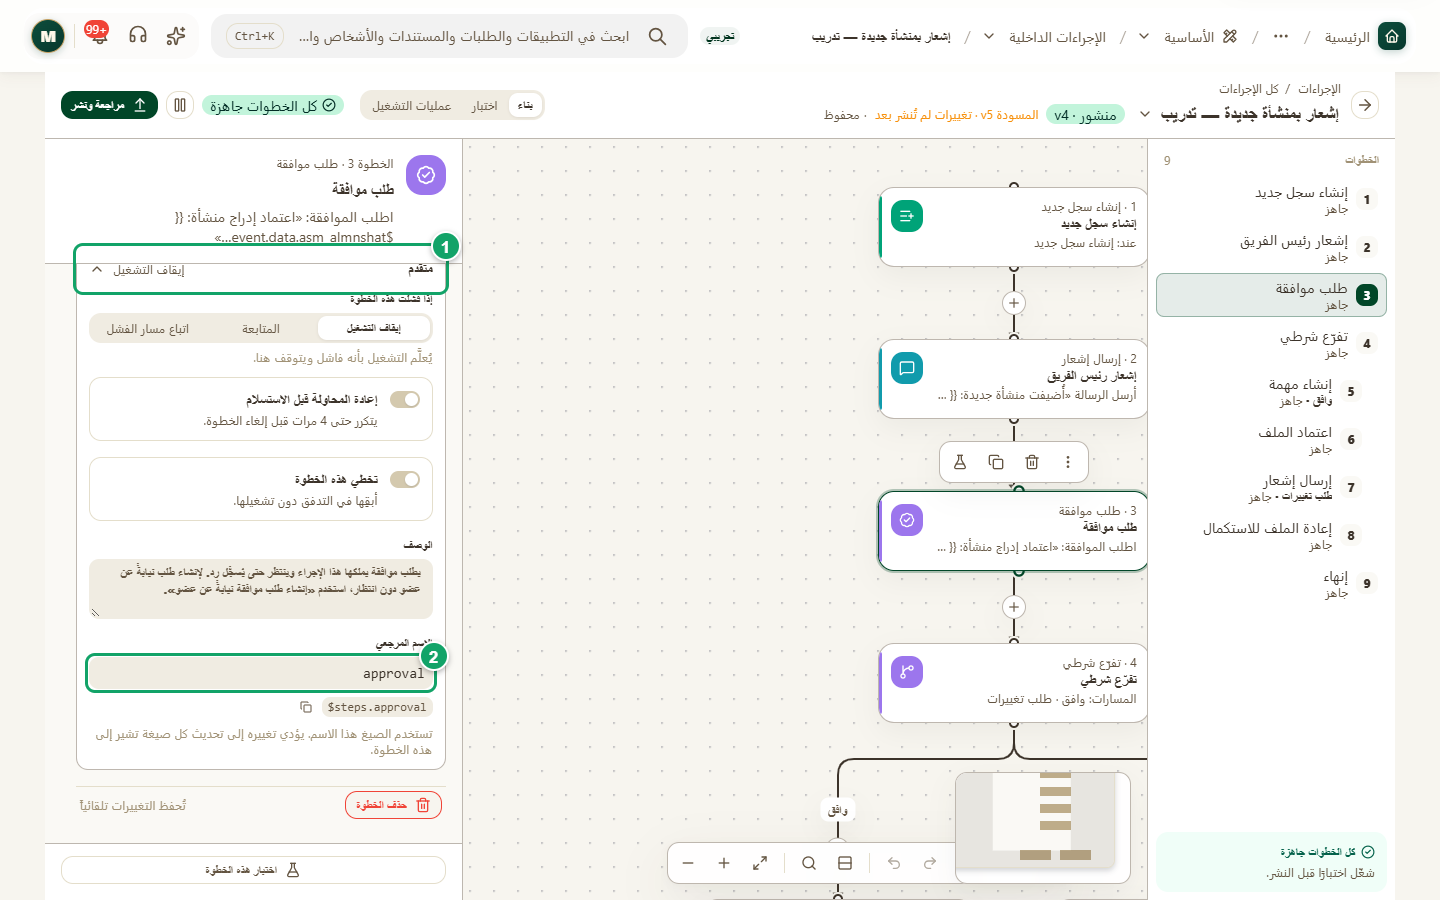
\includegraphics[width=0.95\linewidth]{assets/screens/s3-reference.png}
\caption{الاسم المرجعي لطلب الموافقة}
\label{fig:reference}
\shotnote{الاسم المرجعي لا يظهر لأحد غيرك، لكنه الطريقة الوحيدة لتشير إلى نتيجة هذه الخطوة من خطوة بعدها. اكتبه بأحرف إنجليزية صغيرة دون مسافات. ① «متقدم»: يفتح الإعدادات الإضافية. ② «الاسم المرجعي»: \en{approval}.}
\end{figure}
\textbf{تحقق:} في «الاسم المرجعي» \en{approval}.

\section{المرحلة 3: أضف التفرّع وطريق «وافق»}
\label{sec:branch}
\textbf{لماذا؟} الخطوة العادية يخرج منها طريق واحد. «تفرّع شرطي» يخرج منه أكثر من طريق، ولكل طريق سؤال: «هل رد أحمد بكذا؟». أول طريق: إذا وافق.
\begin{enumerate}
\item اضغط «+» على الخط بين «طلب موافقة» و«إنهاء»، وابحث عن «تفرّع شرطي»، واختره.
\item أبقِ «المسارات المطابقة» على «أول مسار مطابق».
\item تحت «مسارات القرارات» مسار جاهز اسمه \en{Branch 1}. في خانة «التسمية» احذفه واكتب «وافق».
\item بجانب «الشرط» زر التعبير \en{</>}. اضغطه، واحذف ما في الخانة، والصق السطر التالي كما هو:\\
\en{\$steps.approval.output.terminalOutcomeKey == "approved"}
\item اضغط \en{Esc}.
\end{enumerate}

\begin{rcnote}[اقرأ الشرط كجملة]
\en{\$steps.approval} تعني «خطوة approval». و\en{output.terminalOutcomeKey} تعني «النتيجة التي انتهى إليها الطلب». و\en{== "approved"} تعني «تساوي approved». فالجملة كلها: «هل انتهى طلب الموافقة بالموافقة؟».
\end{rcnote}

\begin{figure}[H]
\centering
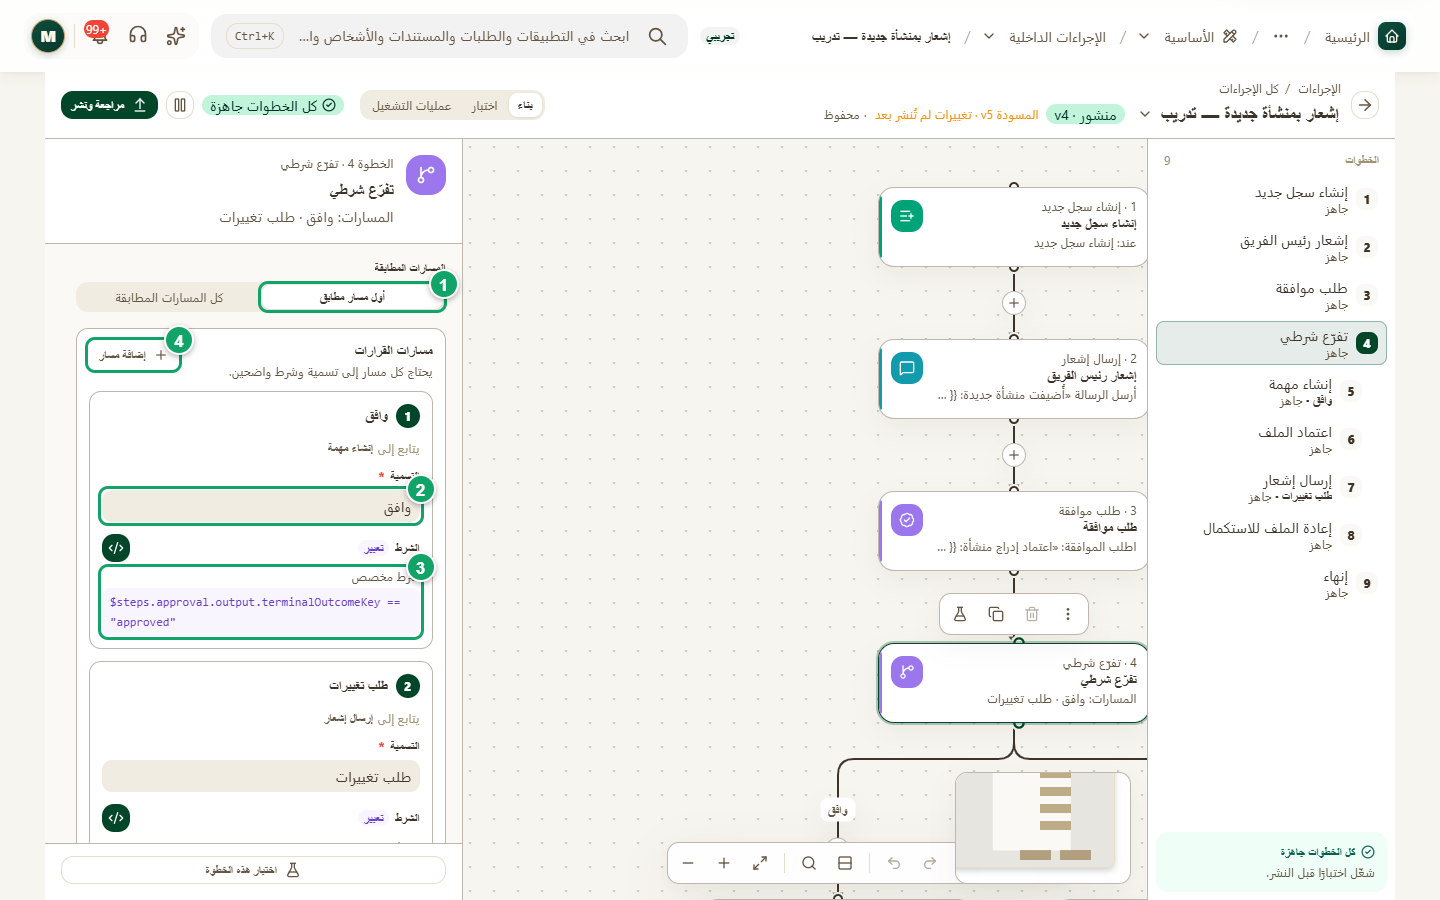
\includegraphics[width=0.95\linewidth]{assets/screens/s3-branch.png}
\caption{إعداد التفرّع}
\label{fig:branch}
\shotnote{لكل مسار تسمية تظهر على الخط في اللوحة، وشرط يُسأل بعد رد أحمد. «يتابع إلى» تحت كل مسار تخبرك بأول خطوة فيه. ① «أول مسار مطابق»: يسلك الإجراء أول طريق يصح شرطه. ② «التسمية»: «وافق». ③ الشرط بعد كتابته. ④ «إضافة مسار».}
\end{figure}
\textbf{تحقق:} تحت المسار الأول «شرط مخصص» ثم الشرط الذي لصقته، ورأس الخطوة يقول «المسارات: وافق».

\section{المرحلة 3: أضف طريق «طلب تغييرات»}
\label{sec:branch-2}
\textbf{لماذا؟} إذا طلب أحمد تغييرات، نريد طريقاً آخر. الشرط نفسه، مع نتيجة الزر الثاني.
\begin{enumerate}
\item اضغط «إضافة مسار».
\item في «التسمية» للمسار الثاني اكتب «طلب تغييرات».
\item اضغط زر التعبير بجانب «الشرط» الثاني، والصق:\\
\en{\$steps.approval.output.terminalOutcomeKey == "needs\_changes"}
\item اضغط \en{Esc}، ثم «ملاءمة سير العمل للعرض» في أسفل اللوحة لترى الإجراء كاملاً.
\end{enumerate}

\begin{figure}[H]
\centering
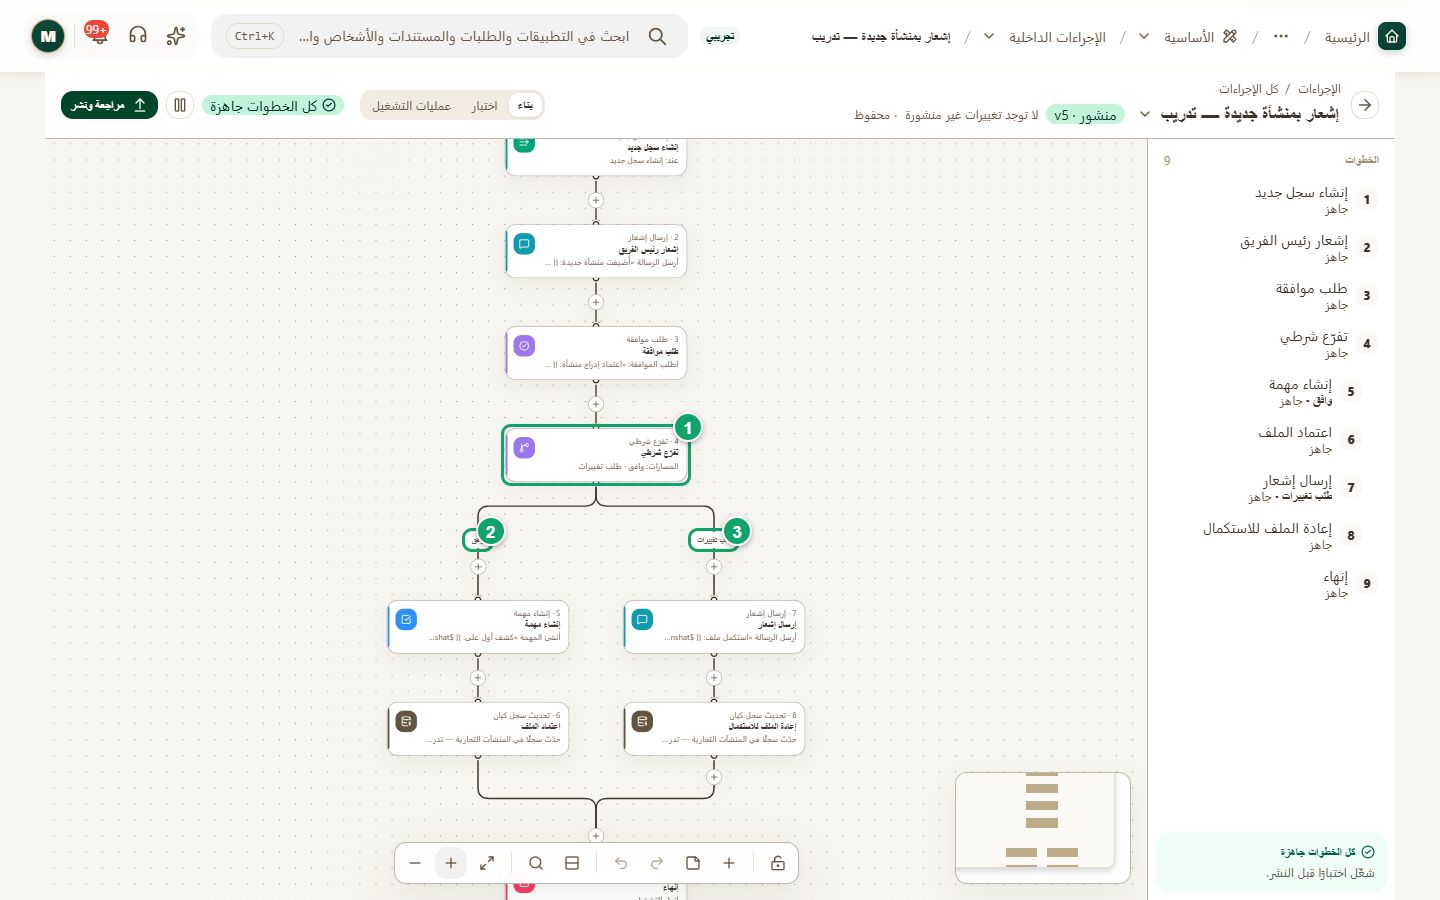
\includegraphics[width=0.95\linewidth]{assets/screens/s3-canvas.png}
\caption{طريقان يخرجان من التفرّع}
\label{fig:canvas}
\shotnote{الصورة بعد المرحلة الرابعة، فترى في كل طريق خطوتيه. بعد إضافة المسار الثاني مباشرة يكون كل طريق فارغاً، ويلتقي الطريقان عند «إنهاء». ① «تفرّع شرطي». ② طريق «وافق». ③ طريق «طلب تغييرات».}
\end{figure}
\textbf{تحقق:} على اللوحة خطّان يخرجان من «تفرّع شرطي»، على الأول «وافق» وعلى الثاني «طلب تغييرات»، ولكل منهما زر «+» خاص به.

\section{المرحلة 4: في طريق «وافق» أنشئ مهمة لنور}
\label{sec:task}
\textbf{لماذا؟} الموافقة قرار، لكنها لا تنفّذ الكشف. المهمة تجعل الكشف عملاً له صاحب يراه في مهامه.
\begin{enumerate}
\item اضغط «+» الذي على طريق «وافق»، وابحث عن «إنشاء مهمة»، واختره.
\item في «عنوان المهمة» اكتب «كشف أول على: »، ثم أدرج اسم المنشأة بـ«إدراج بيانات».
\item انزل إلى «المكلّفون»، واضغط «تحديد»، واختر نور (أو نفسك). اضغط \en{Esc}.
\item اترك بقية الحقول كما هي.
\end{enumerate}

\begin{figure}[H]
\centering
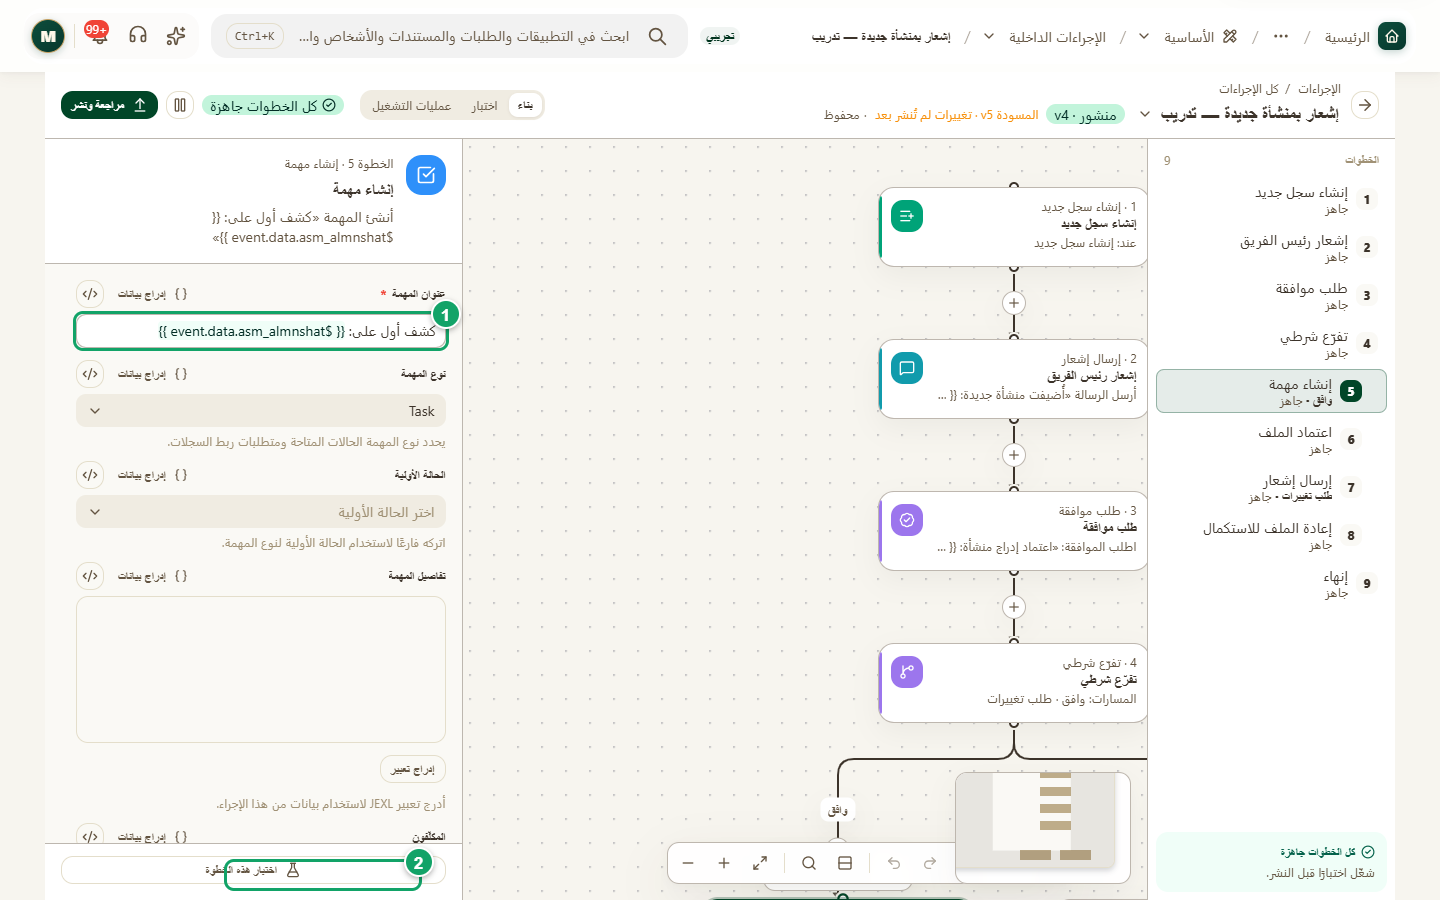
\includegraphics[width=0.95\linewidth]{assets/screens/s4-task.png}
\caption{حقلا المهمة اللذان نحتاجهما}
\label{fig:task}
\shotnote{في خطوة «إنشاء مهمة» حقول كثيرة، لكن المطلوب منها واحد فقط: العنوان. نضيف المكلّف حتى تظهر المهمة عند نور. ① «عنوان المهمة». ② «المكلّفون».}
\end{figure}
\textbf{تحقق:} على طريق «وافق» بطاقة «إنشاء مهمة»، وفي قائمة «الخطوات» تحتها «وافق · جاهز».

\section{المرحلة 4: في طريق «وافق» غيّر حالة الملف}
\label{sec:update}
\textbf{لماذا؟} من يفتح ملف المنشأة يجب أن يرى أنها اعتُمدت، دون أن يبحث عن الطلب. سنكتب «معتمدة للكشف» في «حالة الملف».
\begin{enumerate}
\item اضغط «+» بعد «إنشاء مهمة» على طريق «وافق»، وابحث عن «تحديث سجل كيان»، واختره.
\item غيّر «اسم الخطوة» أعلى اللوحة إلى «اعتماد الملف»، واضغط \en{Enter}.
\item في «الكيان» اختر «المنشآت التجارية».
\item بجانب «السجل» اضغط زر التعبير، واكتب \en{\$event.data.id}، ثم \en{Esc}. معناه: «السجل الذي بدأ الإجراء».
\item تحت «قيم الحقول» اضغط «أضف قيمة الحقل»، واختر «حالة الملف»، ثم اختر في الخانة التي تظهر «معتمدة للكشف».
\end{enumerate}

\begin{figure}[H]
\centering
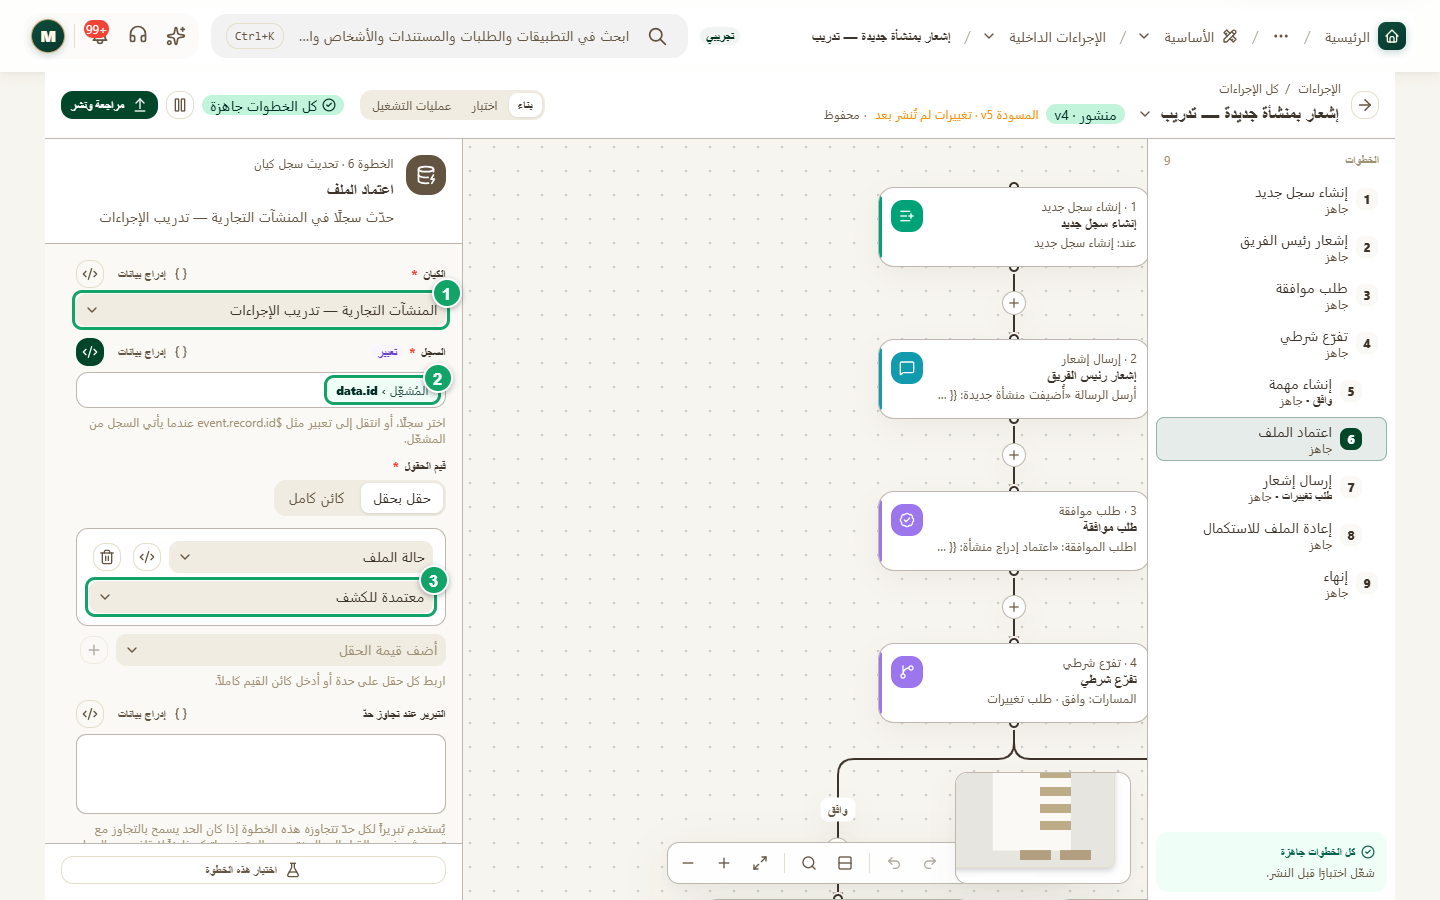
\includegraphics[width=0.95\linewidth]{assets/screens/s4-update.png}
\caption{تحديث حالة الملف}
\label{fig:update}
\shotnote{بعد كتابة التعبير يظهر في «السجل» «المُشغِّل › data.id»؛ أي أن الخطوة ستعدّل المنشأة نفسها التي أُضيفت، لا منشأة ثابتة. ① «الكيان». ② «السجل»: المنشأة التي بدأت الإجراء. ③ القيمة الجديدة لـ«حالة الملف».}
\end{figure}
\textbf{تحقق:} الخطوة «اعتماد الملف» «جاهز»، وتحت «حالة الملف» «معتمدة للكشف».

\section{المرحلة 4: جهّز طريق «طلب تغييرات»}
\label{sec:changes}
\textbf{لماذا؟} إذا طلب أحمد تغييرات، يجب أن يعرف نور، وأن يرى الملف أنه ناقص. نكرر ما تعلمته، بقيم مختلفة.
\begin{enumerate}
\item اضغط «+» على طريق «طلب تغييرات»، وأضف «إرسال إشعار».
\item «عنوان الرسالة»: «استكمل ملف: » ثم اسم المنشأة مُدرجاً. «محتوى الرسالة»: «طلب رئيس الفريق تغييرات. افتح طلب الموافقة لتقرأ ملاحظته، ثم صحّح الملف.» «المستلمون»: نور.
\item اضغط «+» بعد هذا الإشعار، وأضف «تحديث سجل كيان». سمّه «إعادة الملف للاستكمال».
\item املأه كما في الخطوة السابقة: «المنشآت التجارية»، و\en{\$event.data.id}، و«حالة الملف» = «تحتاج استكمالاً».
\end{enumerate}
\textbf{تحقق:} في قائمة «الخطوات» تسع خطوات، كلها «جاهز»، والرأس يقول «كل الخطوات جاهزة».

\section{المرحلة 4: انشر وجرّب الطريقين}
\label{sec:final-run}
\textbf{لماذا؟} الطريق الذي لم يُجرَّب لا تعرف إن كان يعمل. نضيف منشأتين: نوافق على الأولى، ونطلب تغييرات للثانية.
\begin{enumerate}
\item اضغط «مراجعة ونشر» ← «نشر».
\item أضف «فرن القمح — تدريب» و«مطعم الياسمين — تدريب».
\item في «طلبات بانتظارك» افتح طلب «فرن القمح — تدريب»، واضغط «موافقة» ← «تأكيد موافقة».
\item افتح طلب «مطعم الياسمين — تدريب»، واضغط «طلب تغييرات»، واكتب «العنوان التفصيلي ناقص.»، ثم أكّد.
\item افتح «المنشآت التجارية».
\end{enumerate}

\begin{figure}[H]
\centering
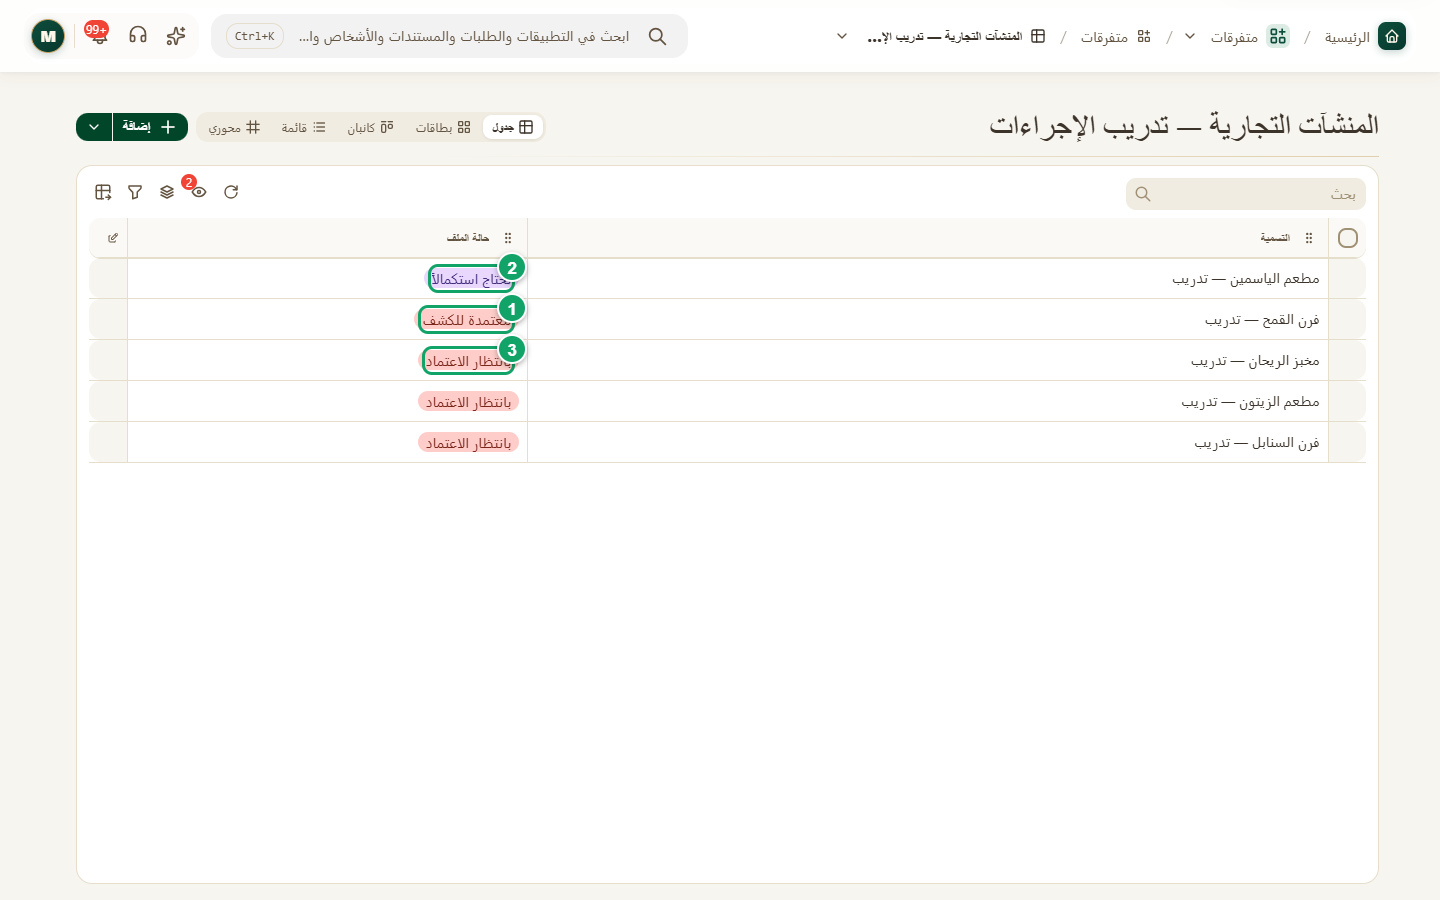
\includegraphics[width=0.95\linewidth]{assets/screens/s4-records.png}
\caption{النتيجة في قائمة المنشآت}
\label{fig:records}
\shotnote{كل منشأة تحمل الآن حالة تحكي ما جرى لها: واحدة اعتُمدت، وواحدة أُعيدت، والمنشآت التي جرّبنا بها المراحل الأولى بقيت «بانتظار الاعتماد» لأن الإجراء لم يكن يغيّر الحالة يومها. ① «معتمدة للكشف»: «فرن القمح — تدريب». ② «تحتاج استكمالاً»: «مطعم الياسمين — تدريب». ③ «بانتظار الاعتماد»: منشآت المراحل الأولى.}
\end{figure}
\textbf{تحقق:} «فرن القمح — تدريب» «معتمدة للكشف»، وفي المهام «كشف أول على: فرن القمح — تدريب». و«مطعم الياسمين — تدريب» «تحتاج استكمالاً»، وفي «المستجدات» «استكمل ملف: مطعم الياسمين — تدريب». في «عمليات التشغيل» عمليتان «مكتمل». أنهيت الإجراء كاملاً.

\section{إذا لم يحدث ما تتوقعه}
\label{sec:troubleshooting}
\textbf{لماذا؟} كل مشكلة في هذا الجدول ظهرت فعلاً أثناء تجربة هذا الفصل. ابحث عن ما رأيته، وطبّق الحل قبل أن تعيد البناء من البداية.
\begin{table}[H]
\centering
\caption{ما رأيته وما تفعله}
\label{tab:troubleshooting}
\begin{tabularx}{\linewidth}{R{4.2cm} Y}
\rcHeaderRow
\thh{ما رأيته} & \thh{ما تفعله}\\
أضفت منشأة ولا توجد أي عملية تشغيل & هل نشرت؟ يجب أن يقول الرأس «منشور». ثم تأكد أن «الجدول» في المشغّل هو جدول المنشأة التي أضفتها.\\
لا أجد الإشعار & افتح الجرس ثم تبويب «المستجدات»، لا «للتنفيذ».\\
«إدراج بيانات» لا يعرض حقولي & أضف منشأة مرة واحدة بعد النشر، ثم ارجع إلى الخطوة؛ تعرض القائمة بيانات آخر تشغيل.\\
العملية «فشل» وفيها «Internal command failed with status 422» & لم تكتب \en{[]} في «مرفقات المكتبة». راجع خطوة المرفقات، ثم انشر وأضف منشأة جديدة.\\
العملية تنتظر ولا تكتمل & هذا طبيعي حتى يرد المعتمد. افتح «طلبات بانتظارك» بحسابه.\\
سلك الإجراء طريقاً غير الذي توقعته & افتح العملية، ثم خطوة «طلب موافقة»، واقرأ \en{terminalOutcomeKey}. قارنها حرفاً بحرف بما كتبته في الشرط.\\
عدّلت الإجراء ولم يتغير شيء & هل نشرت بعد التعديل؟ الرأس يقول «تغييرات لم تُنشر بعد» حتى تنشر.\\
\end{tabularx}
\end{table}
\textbf{تحقق:} قبل أن تطلب مساعدة، دوّن اسم المنشأة، ورقم الإصدار في الرأس، وحالة العملية، ونص الرسالة تحت «التشغيل المحدد».

\section{نفّذ وحدك: تمرين الإتقان}
\label{sec:practice}
\textbf{لماذا؟} تتقن الإجراءات عندما تبني واحداً دون أن تنظر إلى الخطوات. التمرين يضيف ريم إلى الإجراء الذي بنيته.
\begin{enumerate}
\item القاعدة: «بعد أن يوافق أحمد، يصل إلى ريم إشعار بأن المنشأة اعتُمدت.» قل بصوت عالٍ: في أي طريق ستضيف الخطوة؟ ولماذا ليس قبل التفرّع؟
\item أضف الإشعار في المكان الصحيح، وأدرج اسم المنشأة في عنوانه.
\item انشر، وأضف منشأة جديدة، ووافق عليها.
\item افتح عملية التشغيل، وتأكد أن خطوة إشعار ريم «نجح»، وأن خطوات طريق «طلب تغييرات» لم تعمل.
\item أضف منشأة أخرى واطلب لها تغييرات. تأكد أن ريم لم يصلها شيء هذه المرة.
\end{enumerate}

\begin{table}[H]
\centering
\caption{أدلة الإتقان}
\label{tab:acceptance}
\begin{tabularx}{\linewidth}{R{3.8cm} Y}
\rcHeaderRow
\thh{المهارة} & \thh{تعرف أنك أتقنتها عندما…}\\
البناء & أضفت خطوة في المكان الصحيح من أول مرة.\\
البيانات & ظهر اسم المنشأة الحقيقي في الإشعار، لا الرمز بين القوسين.\\
النشر & عرفت من الرأس هل ما تراه منشور أم مسودة.\\
القرار & عرفت أي طريق سيسلكه الإجراء قبل أن تضغط زر الرد.\\
القراءة & فسّرت من عملية التشغيل لماذا لم تعمل خطوة ما.\\
\end{tabularx}
\end{table}

\subsection{ثلاثة أسئلة قبل أن تعدّ نفسك جاهزاً}
\begin{itemize}
\item عدّلت نص الإشعار ولم يتغير ما يصل: لماذا؟ لأنك لم تنشر بعد التعديل.
\item عملية «بانتظار استجابة» منذ يومين: هل هي معطّلة؟ لا؛ تنتظر رد المعتمد، أو انتهاء «المهلة الزمنية».
\item لماذا لا نكتب اسم المنشأة بأيدينا في العنوان؟ لأن الإجراء يعمل لكل منشأة، و«إدراج بيانات» يضع اسم كل منشأة في طلبها.
\end{itemize}
\textbf{تحقق:} أنهيت التمرين، وأجبت عن الأسئلة الثلاثة دون الرجوع إلى الدليل. الفصل التالي يطبّق ما تعلمته على متابعة حقيقية لضبط تمويني.
